\documentclass{vkr}
\usepackage[english, russian]{babel} % переносы
\usepackage{graphicx} % для вставки картинок
\graphicspath{{images/}} % путь к изображениям
\usepackage[hidelinks]{hyperref}
\usepackage{float} % определяет метод H для рисунка с переносом на следующую страницу, ели не помещается
\usepackage{pdflscape}
\addto{\captionsrussian}{\renewcommand{\refname}{СПИСОК ИСПОЛЬЗОВАННЫХ ИСТОЧНИКОВ}}
\usepackage{xltabular} % для вставки таблиц
\usepackage{makecell}
\renewcommand\theadfont{} % шрифт в /thead
\usepackage{array} % для определения новых типов столбцов таблиц
\newcolumntype{T}{>{\centering\arraybackslash}X} % новый тип столбца T - автоматическая ширина столбца с выравниванием по центру
\newcolumntype{R}{>{\raggedleft\arraybackslash}X} % новый тип столбца R - автоматическая ширина столбца с выравниванием по правому краю
\newcolumntype{C}[1]{>{\centering\let\newline\\\arraybackslash\hspace{0pt}}m{#1}} % новый тип столбца C - фиксированная ширина столбца с выравниванием по центру
\newcolumntype{r}[1]{>{\raggedleft\arraybackslash}p{#1}} % новый тип столбца r - фиксированная ширина столбца с выравниванием по правому краю
\newcommand{\centrow}{\centering\arraybackslash} % командой \centrow можно центрировать одну ячейку (заголовок) в столбце типа X или p, оставив в оcтальных ячейках другой тип выравнивания
\newcommand{\finishhead}{\endhead\hline\endlastfoot}
\newcommand{\continuecaption}[1]{\captionsetup{labelformat=empty} \caption[]{#1}\\ \hline }
\usepackage{etoolbox}
\AtBeginEnvironment{xltabular}{\refstepcounter{tablecnt}} % подсчет таблиц xltabular, обычные таблицы подсчитываются в классе

\usepackage[tableposition=top]{caption} % подпись таблицы вверху
\captionsetup{strut=off}
\setlength{\intextsep}{0pt} % Vertical space above & below [h] floats
\setlength{\textfloatsep}{0pt} % Vertical space below (above) [t] ([b]) floats
\DeclareCaptionLabelFormat{gostfigure}{Рисунок #2} %подпись рисунка
\DeclareCaptionLabelFormat{gosttable}{Таблица #2} %подпись таблицы
\DeclareCaptionLabelSeparator{gost}{~--~} %разделитель в рисунках и таблицах
\captionsetup{labelsep=gost}
\captionsetup[figure]{aboveskip=10pt,belowskip=4mm,justification=centering,labelformat=gostfigure} % настройка подписи рисунка
\captionsetup[table]{font={stretch=1.41},skip=0pt,belowskip=0pt,aboveskip=8.5pt,singlelinecheck=off,labelformat=gosttable} % настройка подписи таблицы

\setlength{\LTpre}{8mm} % отступ сверху таблицы
\setlength{\LTpost}{6mm} % отступ снизу таблицы

\usepackage{enumitem}
\renewcommand{\labelitemi}{\textbullet}

\usepackage{enumitem}
\setlist{nolistsep,wide=\parindent,itemindent=*}
\setlist[itemize,2]{label=○}   % отступы вокруг списков, выравнивание с учетом разделителя

\usepackage{color} %% это для отображения цвета в коде
\usepackage{listings} %% листинги кода
\setmonofont[Scale=0.7]{Verdana} % моноширный шрифт для листинга

\definecolor{codegreen}{rgb}{0,0.6,0}
\definecolor{codegray}{rgb}{0.5,0.5,0.5}
\definecolor{codepurple}{rgb}{0.58,0,0.82}

\lstset{ %
language=C,                 % выбор языка для подсветки (здесь это С)
numbers=left,               % где поставить нумерацию строк (слева\справа)
numberstyle=\tiny,           % размер шрифта для номеров строк
stepnumber=1,                   % размер шага между двумя номерами строк
numbersep=5pt,                % как далеко отстоят номера строк от подсвечиваемого кода
commentstyle=\color{codegreen},
keywordstyle=\color{magenta},
numberstyle=\tiny\color{codegray},
stringstyle=\color{codepurple},
basicstyle=\linespread{0.95}\ttfamily,
backgroundcolor=\color{white}, % цвет фона подсветки - используем \usepackage{color}
showspaces=false,            % показывать или нет пробелы специальными отступами
showstringspaces=false,      % показывать или нет пробелы в строках
showtabs=false,             % показывать или нет табуляцию в строках
frame=single,              % рисовать рамку вокруг кода
tabsize=2,                 % размер табуляции по умолчанию равен 2 пробелам
captionpos=t,              % позиция заголовка вверху [t] или внизу [b] 
breaklines=true,           % автоматически переносить строки (да\нет)
breakatwhitespace=false, % переносить строки только если есть пробел
escapeinside={\%*}{*)}   % если нужно добавить комментарии в коде
}

\makeatletter % чтобы допускались русские комментарии в листингах
\lst@InputCatcodes
\def\lst@DefEC{%
 \lst@CCECUse \lst@ProcessLetter
  ^^80^^81^^82^^83^^84^^85^^86^^87^^88^^89^^8a^^8b^^8c^^8d^^8e^^8f%
  ^^90^^91^^92^^93^^94^^95^^96^^97^^98^^99^^9a^^9b^^9c^^9d^^9e^^9f%
  ^^a0^^a1^^a2^^a3^^a4^^a5^^a6^^a7^^a8^^a9^^aa^^ab^^ac^^ad^^ae^^af%
  ^^b0^^b1^^b2^^b3^^b4^^b5^^b6^^b7^^b8^^b9^^ba^^bb^^bc^^bd^^be^^bf%
  ^^c0^^c1^^c2^^c3^^c4^^c5^^c6^^c7^^c8^^c9^^ca^^cb^^cc^^cd^^ce^^cf%
  ^^d0^^d1^^d2^^d3^^d4^^d5^^d6^^d7^^d8^^d9^^da^^db^^dc^^dd^^de^^df%
  ^^e0^^e1^^e2^^e3^^e4^^e5^^e6^^e7^^e8^^e9^^ea^^eb^^ec^^ed^^ee^^ef%
  ^^f0^^f1^^f2^^f3^^f4^^f5^^f6^^f7^^f8^^f9^^fa^^fb^^fc^^fd^^fe^^ff%
  ^^^^20ac^^^^0153^^^^0152%
  % Basic Cyrillic alphabet coverage
  ^^^^0410^^^^0411^^^^0412^^^^0413^^^^0414^^^^0415^^^^0416^^^^0417%
  ^^^^0418^^^^0419^^^^041a^^^^041b^^^^041c^^^^041d^^^^041e^^^^041f%
  ^^^^0420^^^^0421^^^^0422^^^^0423^^^^0424^^^^0425^^^^0426^^^^0427%
  ^^^^0428^^^^0429^^^^042a^^^^042b^^^^042c^^^^042d^^^^042e^^^^042f%
  ^^^^0430^^^^0431^^^^0432^^^^0433^^^^0434^^^^0435^^^^0436^^^^0437%
  ^^^^0438^^^^0439^^^^043a^^^^043b^^^^043c^^^^043d^^^^043e^^^^043f%
  ^^^^0440^^^^0441^^^^0442^^^^0443^^^^0444^^^^0445^^^^0446^^^^0447%
  ^^^^0448^^^^0449^^^^044a^^^^044b^^^^044c^^^^044d^^^^044e^^^^044f%
  ^^^^0401^^^^0451%
  %%%
  ^^00}
\lst@RestoreCatcodes
\makeatother


% Режим шаблона (должен быть включен один из трех)
%\ВКРtrue
\Практикаtrue
%\Курсоваяtrue

\newcommand{\Дисциплина}{<<Проектирование и архитектура программных систем>>} % для курсовой
\newcommand{\КодСпециальности}{09.03.04} % Курсовая
\newcommand{\Специальность}{Программная инженерия} % Курсовая
\newcommand{\Тема}{Разработка web-сайта «Русатом – Аддитивные технологии» на платформе} % ВКР Курсовая
\newcommand{\ТемаВтораяСтрока}{1С-Битрикс}
\newcommand{\ГдеПроводитсяПрактика}{Юго-Западном государственном университете} % для практики
\newcommand{\РуководительПрактПредпр}{Федосов Д. В.} % для практики
\newcommand{\ДолжнРуководительПрактПредпр}{директор} % для практики
\newcommand{\РуководительПрактУнивер}{Чаплыгин А. А.} % для практики
\newcommand{\ДолжнРуководительПрактУнивер}{к.т.н. доцент} % для практики
\newcommand{\Автор}{Р.Д. Попов}
\newcommand{\АвторРод}{Попов Р.Д.}
\newcommand{\АвторПолностьюРод}{Попова Романа Денисовича} % для практики
\newcommand{\Шифр}{хх-хх-хххх}
\newcommand{\Курс}{4 } % для практики
\newcommand{\Группа}{ПО-11б}
\newcommand{\Руководитель}{А. А. Чаплыгин} % для ВКР и курсовой
\newcommand{\Нормоконтроль}{А. А. Чаплыгин} % для ВКР
\newcommand{\ЗавКаф}{А. В. Малышев} % для ВКР
\newcommand{\ДатаПриказа}{«07» апреля 2023~г.} % для ВКР
\newcommand{\НомерПриказа}{1505-с} % для ВКР
\newcommand{\СрокПредоставления}{«13» июня 2023~г.} % для ВКР, курсового

\begin{document}
\maketitle
\ifПрактика{}\else{
   \newpage
\begin{center}
\large\textbf{Минобрнауки России}

\large\textbf{Юго-Западный государственный университет}
\vskip 1em
\normalsize{Кафедра программной инженерии}
\vskip 1em
\ifВКР{
        \begin{flushright}
        \begin{tabular}{p{.4\textwidth}}
        \centrow УТВЕРЖДАЮ: \\
        \centrow Заведующий кафедрой \\
        \hrulefill \\
        \setarstrut{\footnotesize}
        \centrow\footnotesize{(подпись, инициалы, фамилия)}\\
        \restorearstrut
        «\underline{\hspace{1cm}}»
        \underline{\hspace{3cm}}
        20\underline{\hspace{1cm}} г.\\
        \end{tabular}
        \end{flushright}
        }\fi
\end{center}
\vspace{1em}
  \begin{center}
  \large
\ifВКР{
ЗАДАНИЕ НА ВЫПУСКНУЮ КВАЛИФИКАЦИОННУЮ РАБОТУ
  ПО ПРОГРАММЕ БАКАЛАВРИАТА}
  \else
ЗАДАНИЕ НА КУРСОВУЮ РАБОТУ (ПРОЕКТ)
\fi
\normalsize
  \end{center}
\vspace{1em}
{\parindent0pt
  Студента \АвторРод, шифр\ \Шифр, группа \Группа
  
1. Тема «\Тема\ \ТемаВтораяСтрока»
\ifВКР{
утверждена приказом ректора ЮЗГУ от \ДатаПриказа\ № \НомерПриказа
}\fi.

2. Срок предоставления работы к защите \СрокПредоставления

3. Исходные данные для создания программной системы:

3.1. Перечень решаемых задач:}

\renewcommand\labelenumi{\theenumi)}

\begin{enumerate}
\item проанализировать IT-инфраструктуру предприятия;
\item  разработать концептуальную модель системы управления IT-ин\-фра\-струк\-турой предприятия на основе подхода к управлению и организации ИТ-услуг ITSM;
\item спроектировать программную систему управления IT-ин\-фра\-струк\-турой предприятия;
\item сконструировать и протестировать программную систему управления IT-инфраструктурой предприятия.
\end{enumerate}

{\parindent0pt
  3.2. Входные данные и требуемые результаты для программы:}

\begin{enumerate}
\item Входными данными для программной системы являются: данные
справочников комплектующих, конфигураций, ПО, критериев качества SLA,
ИТ-услуг, департаментов компании; технические данные ИТ-ресурсов; данные входящих заявок на ИТ-ресурсы; данные запросов поставщикам на комплектующие.
\item Выходными данными для программной системы являются: сформированные заявки на обслуживание ИТ-ресурсов; сформированные запросы на
закупку комплектующих; сведения о выполненных работах по заявкам; статусы заявок; выходные отчеты (инфографика) – по качеству услуг, по состоянию ИТ-ресурсов, по деятельности ИТ-отдела, по стоимости обслуживания
ИТ-ресурсов, воронка заявок.
\end{enumerate}

{\parindent0pt

  4. Содержание работы (по разделам):
  
  4.1. Введение.
  
  4.1. Анализ предметной области.
  
4.2. Техническое задание: основание для разработки, назначение разработки,
требования к программной системе, требования к оформлению документации.

4.3. Технический проект: общие сведения о программной системе, проект
данных программной системы, проектирование архитектуры программной системы, проектирование пользовательского интерфейса программной системы.

4.4. Рабочий проект: спецификация компонентов и классов программной системы, тестирование программной системы, сборка компонентов программной системы.

4.5. Заключение.

4.6. Список использованных источников.

5. Перечень графического материала:

\списокПлакатов

\vskip 2em
\begin{tabular}{p{6.8cm}C{3.8cm}C{4.8cm}}
Руководитель \ifВКР{ВКР}\else работы (проекта) \fi & \lhrulefill{\fill} & \fillcenter\Руководитель\\
\setarstrut{\footnotesize}
& \footnotesize{(подпись, дата)} & \footnotesize{(инициалы, фамилия)}\\
\restorearstrut
Задание принял к исполнению & \lhrulefill{\fill} & \fillcenter\Автор\\
\setarstrut{\footnotesize}
& \footnotesize{(подпись, дата)} & \footnotesize{(инициалы, фамилия)}\\
\restorearstrut
\end{tabular}
}

\renewcommand\labelenumi{\theenumi.}

   \abstract{РЕФЕРАТ}

Объем работы равен \formbytotal{lastpage}{страниц}{е}{ам}{ам}. Работа содержит \formbytotal{figurecnt}{иллюстраци}{ю}{и}{й}, \formbytotal{tablecnt}{таблиц}{у}{ы}{}, \arabic{bibcount} библиографических источников и \formbytotal{числоПлакатов}{лист}{}{а}{ов} графического материала. Количество приложений – 2. Графический материал представлен в приложении А. Фрагменты исходного кода представлены в приложении Б.

Перечень ключевых слов: аугментация изображений, компьютерное зрение, нейронные сети, Python, OpenCV, Albumentations, геометрические преобразования, цветовые искажения, шум, графический интерфейс, пакетная обработка, машинное обучение, данные, интеллектуальные системы.

Объектом разработки являются автоматизированные системы обработки и распознавания изображений.

Предметом исследования является разработка программы для размножения и аугментации изображений с графическим интерфейсом для компании ООО «Предприятие ВТИ-Сервис». 

Целью выпускной квалификационной работы является повышение эффективности обучения нейронных сетей за счет автоматизированной генерации разнообразных обучающих данных.

В процессе создания программы были выделены ключевые типы аугментаций (геометрические, цветовые, шумовые) через создание соответствующих модулей обработки изображений. Реализованы классы и методы для управления параметрами преобразований (угол поворота, уровень шума, коэффициент контраста), а также разработан механизм пакетной обработки, обеспечивающий корректную работу с малыми наборами данных (менее 10 изображений). Создан интерфейс для настройки уровней аугментации (1×25, 1×50, 1×100) и предпросмотра результатов. Дополнительно реализован функционал экспорта обработанных изображений в стандартных форматах (PNG, JPEG).

Для разработки использованы: язык программирования Python, библиотеки OpenCV и PyQt.

Разработанный сайт был успешно внедрен в компании.

\selectlanguage{english}
\abstract{ABSTRACT}
  
The volume of work is \formbytotal{lastpage}{page}{}{s}{s}. The work contains \formbytotal{figurecnt}{illustration}{}{s}{s}, \formbytotal{tablecnt}{table}{}{s}{s}, \arabic{bibcount} bibliographic sources and \formbytotal{числоПлакатов}{sheet}{}{s}{s} of graphic material. The number of applications is 2. The graphic material is presented in annex A. The layout of the site, including the connection of components, is presented in annex B.

List of keywords: image augmentation, computer vision, neural networks, Python, OpenCV, Albumentations, geometric transformations, color distortions, noise, GUI, batch processing, machine learning, data, intelligent systems.

The object of the research is an image augmentation software with a graphical interface for ООО «Предприятие ВТИ-Сервис».

The object of the development is to improve the training efficiency of neural networks through automated generation of diverse training data.


In the development process, key augmentation types (geометрические, цветовые, шумовые) were implemented through dedicated image processing modules. The system includes classes and methods for transformation parameter control (rotation angle, noise level, contrast ratio) along with a batch processing mechanism that ensures proper operation with small datasets (under 10 images). The interface allows configuring augmentation levels (1×25, 1×50, 1×100) and previewing results. Additionally, the export functionality for processed images in standard formats (PNG, JPEG) has been implemented.

The developed website was successfully implemented in the company.
\selectlanguage{russian}
}\fi
\tableofcontents
\section*{ОБОЗНАЧЕНИЯ И СОКРАЩЕНИЯ}

ИС -- информационная система.

ИТ -- информационные технологии. 

КТС -- комплекс технических средств.

ПО -- программное обеспечение.

РП -- рабочий проект.

ТЗ -- техническое задание.

ТП -- технический проект.

ИНС -- искусственные нейронные сети.

СНС -- сверхточная нейронная сеть.
\ifПрактика{}\else{\section*{ВВЕДЕНИЕ}
\addcontentsline{toc}{section}{ВВЕДЕНИЕ}

Методы компьютерного зрения и глубокого обучения стали неотъемлемой частью современных интеллектуальных систем. Однако их эффективность напрямую зависит от объема и качества обучающих данных. Аугментация изображений — ключевой инструмент для решения проблемы нехватки данных, позволяя искусственно расширять выборки за счет преобразований (геометрических, цветовых, шумовых). Интенсивное развитие нейронных сетей, особенно в областях медицины, автономного транспорта и спутникового мониторинга, требует универсальных программных решений для генерации разнообразных данных.

Аугментация предполагает автоматизированное создание вариаций изображений без изменения их семантического содержания, в отличие от ручного сбора дополнительных данных. Современные библиотеки (например, Albumentations, OpenCV) предоставляют технические возможности для таких преобразований, но их использование часто требует навыков программирования.

Современные ИТ-тренды показывают, что автоматизация подготовки данных — обязательный этап в pipeline машинного обучения. Программа для аугментации становится «лицом» процесса обработки изображений, так как именно она превращает ограниченные исходные данные в пригодные для обучения модели. Это напрямую влияет на точность и надежность интеллектуальных систем.

\emph{Цель настоящей работы} — разработка программы аугментации изображений с графическим интерфейсом для повышения эффективности обучения нейронных сетей. Для достижения цели необходимо решить \emph{следующие задачи}:
\begin{itemize}
	\item провести анализ методов аугментации и их применимости в задачах компьютерного зрения;
	\item разработать техническое задание на ПО, учитывающее требования пользователей;
	\item спроектировать архитектуру программы с поддержкой пакетной обработки и настройки параметров;
	\item реализовать программу на Python с использованием библиотек OpenCV и PyQt;
\end{itemize}

\emph{Структура и объем работы.} Отчёт состоит из введения, трёх разделов основной части, заключения, списка использованных источников и приложений. Общий объём работы — \formbytotal{lastpage}{страниц}{у}{ы}{}.

\emph{Во введении} обоснована актуальность темы, сформулированы цель и задачи работы, описана её структура.

\emph{В первом разделе} проведён анализ предметной области: рассмотрены принципы работы нейронных сетей, методы аугментации изображений и их применение в прикладных задачах (медицина, агротехнологии, безопасность).

\emph{Во втором разделе} представлено техническое задание на разработку программы, включая требования к интерфейсу, функционалу (загрузка изображений, выбор уровня аугментации, предпросмотр) и данным.

\emph{В третьем разделе} описаны проектные решения: выбор технологий (Python, OpenCV), конфигурация уровней аугментации (1×25, 1×50, 1×100) и реализация модулей.

В \emph{заключении} подведены итоги работы, оценена практическая значимость программы и направления её дальнейшего развития.

В \emph{приложении А} приведены примеры аугментированных изображений.
В \emph{приложении Б} представлены фрагменты исходного кода программы. 
}\fi
\section{Анализ предметной области}
\subsection{Искусственные нейронные сети}
\subsubsection{Понятие и принципы работы нейронных сетей}

Искусственные нейронные сети (ИНС) – это один из ключевых инструментов современного машинного обучения, вдохновлённый устройством и работой биологических нейронных структур. Основная идея заключается в построении математических моделей, способных выявлять сложные зависимости в данных и обучаться на примерах без явного программирования логики поведения. 

Базовым элементом искусственной нейронной сети является нейрон – вычислительный узел, который получает на вход числовые значения, применяет к ним весовые коэффициенты, суммирует результат и пропускает его через нелинейную функцию активации. Это позволяет сети моделировать нелинейные зависимости и принимать решения на основе сложных входных данных.


\begin{figure}[H]
	\centering
	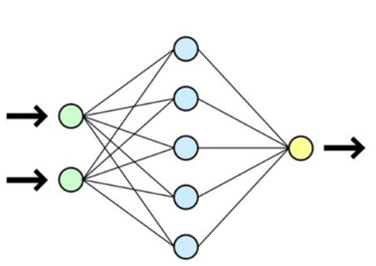
\includegraphics[width=0.7\linewidth]{images/ins}
	\caption{Структура ИНС}
	\label{fig:augexample}
\end{figure}


Типичная структура ИНС (рис. 1) включает:

\begin{itemize}
	\item входной слой, принимающий данные (зелёный цвет);
	\item cкрытые слои, в которых происходит обработка информации (синий цет);
	\item выходной слой, формирующий ответ сети. (желтый цвет).
\end{itemize}


Процесс обучения нейронной сети заключается в подборе весов связей между нейронами таким образом, чтобы минимизировать ошибку между прогнозируемым и фактическим значением. Наиболее распространённым методом оптимизации является обратное распространение ошибки (backpropagation) в сочетании с градиентным спуском.


Нейронные сети бывают различных типов: полносвязные (Dense), сверточные (CNN), рекуррентные (RNN), трансформеры и др. Выбор архитектуры зависит от специфики задачи: для обработки изображений наиболее эффективными зарекомендовали себя сверточные сети, в то время как для анализа последовательностей – рекуррентные и трансформерные модели.

\subsubsection{История и этапы развития нейронных сетей}

Развитие искусственных нейронных сетей прошло несколько ключевых этапов, каждый из которых сопровождался как периодами энтузиазма, так и спадом интереса – так называемыми «зимами искусственного интеллекта».

\begin{enumerate}
	\item Этап зарождения (1940-1960-е гг.):
	
	Первые попытки формализации идей нейронных вычислений относятся к 1943 году, когда Уолтер Питтс и Уоррен МакКаллок представили логико-математическую модель искусственного нейрона. Эта модель, хотя и была простой, заложила фундамент для дальнейших исследований. В 1958 году Фрэнк Розенблатт разработал перцептрон – первую обучаемую нейросеть, способную распознавать простые шаблоны. Однако перцептрон имел ограничения: он не мог решать задачи, в которых классы не разделимы линейно (например, задачи XOR).
	
	\item Первая зима ИИ и застой (1970-1980-е гг.):
	
	После публикации книги Марвина Минского и Сеймура Пейперта Perceptrons (1969), в которой были подробно описаны ограничения перцептрона, интерес к нейросетям значительно снизился. Отсутствие мощных вычислительных ресурсов и недостаток качественных алгоритмов обучения также сыграли свою роль.
	
	\item Возрождения интереса (1986-1990-е гг.):
	
	Ситуация изменилась с появлением алгоритма обратного распространения ошибки (Rumelhart et al., 1986), позволившего эффективно обучать многослойные нейросети. Это открыло путь к построению глубоких моделей. В 1990-е годы нейросети начали использоваться в таких задачах, как распознавание речи, текста и образов.
	
	\item Рождение глубинного обучения (2006-2012 гг.):
	
	Ключевым прорывом стало появление термина «глубинное обучение» (deep learning). Работы Хинтона, Бенжио и Лекуна по автоэнкодерам, сверточным сетям и другим архитектурам позволили строить действительно глубокие модели. В 2012 году модель AlexNet (Крижевский, Хинтон, Суцкевер) выиграла соревнование ImageNet с существенным отрывом, доказав преимущество глубоких сверточных сетей в компьютерном зрении.
	
	\item Современный этап (с 2012 года по настоящее время):
	
	Современные нейросетевые архитектуры (ResNet, EfficientNet, Vision Transformer и др.) достигли впечатляющих результатов в ряде областей – от медицины и автомобильной промышленности до генерации текста и изображений. Развитие специализированных вычислительных платформ (GPU, TPU), доступ к большим данным, а также совершенствование алгоритмов оптимизации сделали обучение сложных моделей доступным и эффективным. Особое внимание уделяется архитектурам с возможностью генерации: GAN, VAE, диффузионные модели и др.
	Таким образом, развитие ИНС представляет собой череду теоретических открытий, технических прорывов и практических применений, которые в совокупности сформировали современный облик машинного обучения.
	
\end{enumerate}

\subsubsection{Современные направления и области применения}

На текущем этапе искусственные нейронные сети (ИНС) стали неотъемлемой частью широкого спектра прикладных и исследовательских задач. Рост вычислительных мощностей, развитие алгоритмов и доступность больших наборов данных способствовали формированию нескольких ключевых направлений применения нейросетевых технологий.

\begin{enumerate}
	\item Обработка изображений и видео.
	
	Сверточные нейронные сети (Convolutional Neural Networks, CNN) обеспечили революцию в компьютерном зрении. Они успешно применяются для:
	
	\begin{itemize}
		\item классификация изображений (ImageNet, CIFAR);
		\item выделения объектов (segmentation);
		\item обнаружения объектов (YOLO, SSD);
		\item распознавания лиц и эмоций;
		\item построения 3D-реконструкций;
		\item восстановления изображений и суперразрешения.
	\end{itemize}
	
	\item Обработка естественного языка (NLP).
	
	Модели трансформерного типа (Transformer, BERT, GPT) позволили достигнуть прорывных результатов в:
	
	\begin{itemize}
		\item машинном переводе;
		\item генерации текста;
		\item извлечении информации;
		\item распознавания лиц и эмоций;
		\item классификации и анализе тональности;
		\item ответах на вопросы и диалоговых системах.
	\end{itemize}
	
	\item Задачи генерации.
	
	Развитие генеративных моделей (в том числе GAN, VAE, Diffusion) дало мощный импульс в таких задачах, как:
	
	\begin{itemize}
		\item генерация фотореалистичных изображений;
		\item стилизация и изменение изображений;
		\item создание видео и 3D-моделей;
		\item распознавания лиц и эмоций;
		\item генерация медицинских снимков для расширения выборок.
	\end{itemize}
	
	\item Медицина.

ИНС используется для анализа рентгеновских снимков, КТ и МРТ, распознавания патологий, поддержки принятия клинических решений. Важное преимущество – способность выявлять паттерны, неочевидные для врача.

	\item Автономный транспорт.
	
Нейросети активно применяются в задачах компьютерного зрения и принятия решений в автономных автомобилях: распознавание дорожных знаков, пешеходов, разметки, прогнозирование траекторий движения.

	\item Финансовый сектор.
	
ИНС используются для прогнозирования временных рядов, обнаружения аномалий (в том числе мошенничества), анализа клиентского поведения и автоматизации поддержки.

	\item Робототехника и промышленность.

Интеллектуальные системы управления, техническое зрение, обработка сигналов с датчиков и предиктивное обслуживание оборудования – все это активно использует нейросети.

	\item Искусство и творчество.

Нейросети генерируют музыку, изображения, видео, стихи и даже сценарии. Развития креативного ИИ расширяет горизонты взаимодействия человека с технологиями.

Таким образом, ИНС охватывают почти все сферы деятельности – от научных исследований до повседневных пользовательских решений. Их универсальность, способность к обучению и высокая точность делают нейросети одним из наиболее перспективных направлений и области ИИ.
	
\end{enumerate}

\subsubsection{Технические ограничения и вызовы при обучении нейронных сетей}

Обучение искусственных нейронных сетей (ИНС) сталкивается с рядом технических ограничений, которые влияют на их эффективность и практическую применимость. Эти вызовы особенно актуальны в условиях ограниченных ресурсов и данных, что делает аугментацию изображений важным инструментом для их преодоления.

\begin{enumerate}
	\item Вычислительные ресурсы:
	
	Современные глубокие нейронные сети требуют значительных вычислительных мощностей, таких как графические процессоры (GPU) или тензорные процессоры (TPU). Отсутствие доступа к таким ресурсам ограничивает масштабируемость моделей, особенно для малого и среднего бизнеса.
	\item Переобучение и недостаток данных: 
	
	При малом объеме обучающих данных ИНС склонны к переобучению, запоминая специфические особенности тренировочной выборки вместо обобщения. Это особенно заметно в задачах с редкими классами или специфическими объектами.
	\item Качество разметки: 
	
	Ошибки в разметке или ее неполнота могут привести к снижению точности модели. Ручная разметка требует значительных затрат времени и ресурсов, особенно в специализированных областях, таких как медицина.
	\item Роль аугментации:
	
	Аугментация изображений позволяет искусственно увеличивать объем данных, улучшать их разнообразие и снижать зависимость от точности разметки. Например, добавление шума или поворотов помогает модели адаптироваться к реальным условиям без необходимости сбора новых данных.
\end{enumerate}

Эти ограничения подчеркивают актуальность разработки программных решений, таких как описываемая в данной работе система аугментации, которая делает обучение ИНС более доступным и эффективным.

\subsubsection{Генеративные нейронные сети}

Генеративные нейронные сети (Generative Neural Networks) представляют собой класс моделей, способных создавать новые дополнительные данные, статистически схожие с исходным обучающим распределением. В контексте обработки изображений эти модели предназначены для генерирования реалистичных изображений, модифицировать существующие, выполнять стилизацию и вносить искажения, полезные для задач аугментации. На рисунке 1.2 представлены базовые афинные преобразования, используемые в аугментации изображения.

\begin{figure}[H]
	\centering
	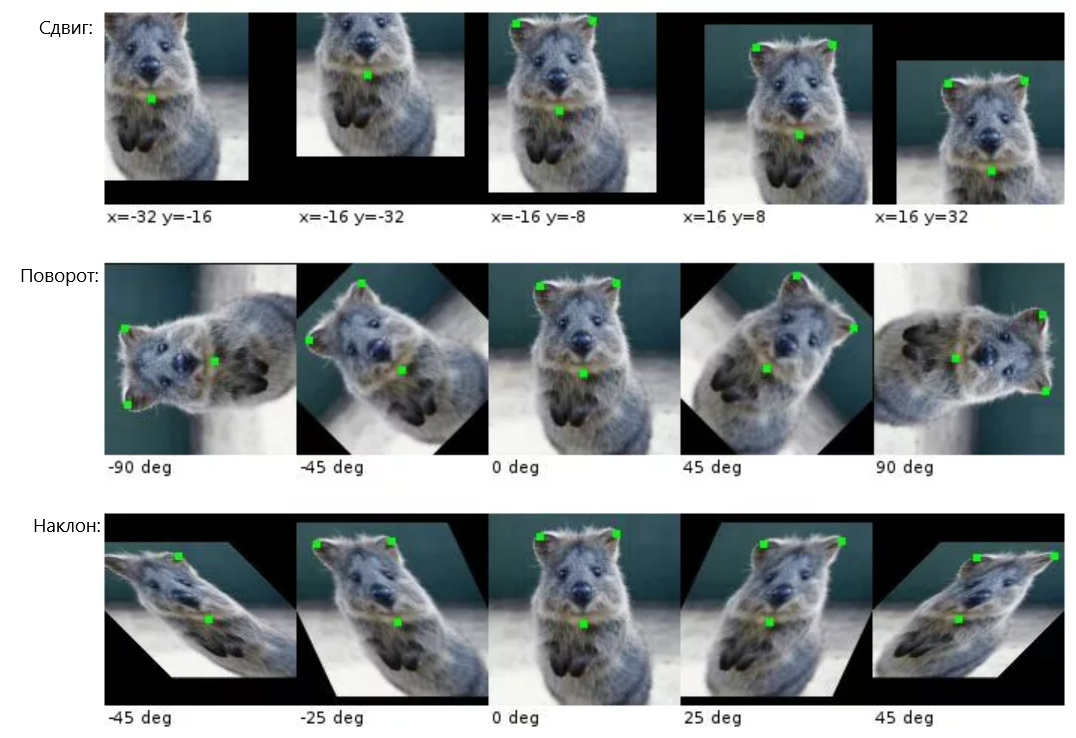
\includegraphics[width=1\linewidth]{images/augexample}
	\caption{Базовые виды аугментации}
	\label{fig:augexample}
\end{figure}


В настоящее время широко используется модель GAN (Generative Neural Networks), которая была предложена Иэном Гудфеллоу в 2014 году. Она состоит из двух нейросетей:

\begin{itemize}
	\item генератор (G) создает изображения на основе случайного шума;
	\item дискриминатор (D) оценивает, являются ли изображения настоящими (из обучающей выборки) или сгенерированными.
\end{itemize}

Обе сети обучаются одновременно при этом генератор стремится обмануть дискриминатор, а дискриминатор – распознать подделку. Такая состязательная структура позволяет достичь высокого качества сгенерированных изображений.

Внедрение в различные области исследований современных технологий привело к разработке разновидностей GAN:
\begin{itemize}
	\item DCGAN – архитектура, основанная на сверточныхнейронных сетях (СНС), применяемая в задачах генерации изображений;
	\item StyleGAN / StyleGAN2 – позволяет управлять стилевыми характеристиками изображения (широко используется в DeepFake, генерации лиц);
	\item CycleGAN – используется для преобразования изображений между двумя доменами без необходимости в парных данных (например, стиль «зима – лето»).
\end{itemize}

Вышеизложенное свидетельствует о том, что технологии GAN находят широкое применение в аугментации объема информации, в тех случаях, когда необходимо увеличить разнообразие изображений сохраняя структуру или стиль.

\textbf{Диффузионные модели}

Одно из наиболее перспективных направлений	 - диффузионные модели (Diffusion Models). В отличие от GAN, они обучаются на задаче поэтапного восстановления изображения из шума.

Процесс включает:

\begin{itemize}
	\item форвард-процесс, где изображение постепенно разрушается путём добавления шума;
	\item реверсивный процесс, где модель обучается восстанавливать изображения обратно шаг за шагом.
\end{itemize}
Примеры моделей:

\begin{itemize}
	\item DDPM (Denoising Diffusion Probabilistic Models) – базовая модель;
	\item Stable Diffusion – открытая и производительная модель для генерации изображений по текстовому описанию;
	\item Imagen / DALLE 2 – модели с высоким качеством генерации, поддерживающие кроссмодальный ввод (текст - изображение).
\end{itemize}

Преимущество применения диффузионных моделей заключается в высокой стабильности и точности при генерации, а также контроле над семантикой изображения. Диффузионные модели активно применяются для синтеза данных в задачах медицинской визуализации и различных технических областях, в которых важно сохранить реалистичность и структурную достоверность. Это свидетельствует о разработке специальных программных средств таких как:

\begin{itemize}
	\item DeepFake – выполняет синтез лиц на основе GAN, используемый как в развлекательной, так и в судебной экспертизе (в том числе для распознавания подделок);
	\item ProGAN / StyleGAN – применяется для генерации лиц высокой реалистичности, включая создание «несуществующих людей»;
	\item CycleGAN для медицины – используется для переноса изображений между различными режимами визуализации (например, МРТ - КТ);
	\item Med-DDPM – диффузионные модели, адаптированные для синтеза медицинских изображений (патологии, опухоли).
\end{itemize}

Таким образом, генеративные нейросети являются мощным инструментом не только в создании новых изображений, но и в аугментации обучающих выборок, особенно в условиях ограниченного объема исходных реальных изображений.

\subsection{Аугментация изображений}
\subsubsection{Понятие аугментации и её цели}

Аугментация изображений (image augmentation) – представляет собой совокупность методов искусственного увеличения обучающей выборки путём модификации исходных изображений без изменения их семантического содержания. Данная технология играет ключевую роль в задачах машинного обучения, связанных с обработкой изображений, поскольку позволяет повысить обобщающую способность моделей, особенно в условиях ограниченных объемов данных.

Основные цели аугментации изображений:

\begin{itemize}
	\item увеличение объема обучающих изображений – позволяет эффективно использовать ограниченный набор исходных изображений, генерируя из них множество вариаций;
	\item снижение переобучения (overfitting) осуществляется за счёт разнообразия входных данных и нейросеть не «запоминает» конкретные изображения, а учится выделять обобщённые признаки;
	\item повышение устойчивости к шумам и искажениям – особенно актуально в реальных условиях, когда изображения могут содержать артефакты, быть смещёнными, плохо освещёнными и т.п.;
	\item имитация реальных условий эксплуатации – например, поворот, масштабирования и сдвиг предназначены для моделирования различных ракурсов и условий съёмки объектов;
	\item балансировка классов в выборке – используется при дисбалансе классов, способствует дополнительнму генерированию изображений в случаях недостаточно представленных категорий;
	\item поддержка робастности – особенно важна в медицинских исследованиях, промышленности и других критичных областях, в которых реализуемые модели должна сохранять точность при отклонениях в данных.
\end{itemize}

Аугментация может применяться как на этапе подготовки данных (оффлайн), так и на динамических этапах во время обучения (онлайн) НС. , Применение этого метода обеспечивает дополнительный объем и разнообразие данных в процессе обучения модели.

Методы аугментации условно делятся на:

\begin{itemize}
	\item классические – основаны на геометрических и цветовых преобразованиях;
	\item генеративные – базируются на нейросетевых моделях, таких как GAN и диффузионные сети.
\end{itemize}

\subsubsection{Методы аугментации изображений}

Классические методы аугментации изображений представляют собой предопределённые трансформации, которые изменяют изображение определённым образом без изменения его смыслового содержания и принадлежности одной генеральной совокупности данных. Эти методы не требуют обучения и широко применяются в промышленности и научных исследованиях благодаря простоте реализации и эффективности.

\paragraph{Геометрические преобразования}

Геометрические преобразования являются одним из наиболее распространённых методов, применяемых в случаях недостаточной информации об анализируемых изображениях со сложной структурой объектов.

Основные афинные преобразования, используемые при изменении положения, ориентации и масштаба объектов на изображении заключаются в следующем:

\begin{itemize}
	\item поворот: изображение поворачивается на случайный или определенный заданный угол, обычно в пределах от -30 до +30 градусов. Это позволяет нейросети быть устойчивой к изменениям угла обзора;
	\item сдвиг пикселей изображения: изображение смещается по горизонтали или вертикали. Сдвиги до 10-20 процентов от размера изображения сохраняют информативность, но создают необходимое разнообразие;
	\item масштабирование: меняется масштаб изображения, как с увеличением, так и с уменьшением. Важно сохранять объект полностью в кадре, чтобы не потерять ключевые признаки;
	\item обрезка: выбирается случайная или центральная часть изображения. Позволяет сделать модель устойчивой к частичному отсутствию информации;
	\item отражение: зеркальное отображение по горизонтали и/или вертикали. Эффективно для симметричных объектов (лица, животные, транспорт);
	\item искажение (Shearing, Affine/Perspective transforms).
\end{itemize}

Геометрические искажения формы объекта, целесообразно применять для моделирования наклонов и перспективных изменений. Геометрические преобразования наиболее эффективных в задачах, где важна пространственная инвариантность – например, в распознавании объектов, медицинской диагностике, анализе сцен.

\paragraph{Цветовые и яркостные искажения}

Изменение цветовых и яркостных искажений предоставляют возможность имититации изменений условий освещения, качества съёмки, особенностей сенсоров и других факторов, влияющих на внешний вид изображения, но не на его семантику. Эти методы повышают устойчивость модели к разнообразным фотометрическим условиям, которые встречаются в реальных данных. Распространенной методикой исследований являются:

\begin{itemize}
	\item изменение яркости: добавление или вычитания значения ко всем пикселям изображения. Позволяет адаптировать модель к условиям пере- или недоэкспонированных снимков;
	\item изменение контрастности: изменение различия между яркими и тёмными участками. Повышает способность модели работать с изображениями разного качества;
	\item изменение насыщенности: управление интенсивностью цвета. При снижении насыщенности изображение приближается к чёрно-белому, что проверяет устойчивость модели к отсутствию цветовой информации;
	\item цветовые преобразования в разных пространствах (HSV, LAB и др.): выполняются преобразования изображения в альтернативные цветовые пространства, где проще и управляемее вносить изменения в яркость, тон и насыщенность;
	\item гамма-коррекция изображений: моделирует особенности различных дисплеев и сенсоров.
\end{itemize}

\paragraph{Шум, искажения, маскирование}

Данная группа методов направлена на повышение устойчивости моделей к частичным повреждениям, шумам и отсутствию информации на изображении. Это особенно актуально для систем, которые функционируют в условиях нестабильного качества входных данных: например, при съёмке на мобильные устройства, в условиях плохой освещённости или при наличии физических повреждений сенсоров.

Для моделирования и отображения подобной информации чаще всего применяют методы:

\begin{enumerate}
	\item Добавление различного вида шумов на изображения таких как:
	\begin{itemize}
	\item гауссов шум: добавление случайных значений, сгенерированных про нормальное распределение, ко всем или части пикселей изображения;
	\item шум «соль и перец»: случайная замена отдельных пикселей на чёрный или белый цвет;
	\item шум Пуассона, спекл-шум и др.: моделируют особенности определённых сенсоров.
	\end{itemize}
	\item Размытие изображений:
	\begin{itemize}
	\item гауссово размытие: мягкое сглаживание изображения, может имитировать расфокус;
	\item размытие в движении: имитация движения камеры или объекта;
	\item медианное: используется для удаления шумов и проверки устойчивости к потере деталей.
	\end{itemize}
	\item Маскирование изображений: случайное зануление или закрашивание фрагментов изображения (например, прямоугольных областей). Это заставляет модель опираться на контекст и не переобучаться на отдельные детали.
	\item JPEG-сжатие: умышленное снижение качества изображения, чтобы повысить устойчивость модели к потерям информации, характерным для изображений в интернете и мессенджерах.
	\item Объединённые методы деградации: комбинация шумов, искажений и потерь качества, имитирующая реальные «грязные» данные – особенно важно при обучении моделей для работы в полевых условиях.
\end{enumerate}

Построенные на основе методов аугментации изображений интеллектуальные системы предназначены для применения в различных областях исследований.

\subsection{Актуальность темы}

Качество и объём обучающей выборки – один из определяющих факторов успеха в обучении нейронных сетей, особенно в задачах компьютерного зрения. Модели глубокого обучения требуют большого количества разнообразных, достоверно размеченных данных, чтобы эффективно обобщать знания и демонстрировать высокую точность на ранее не виденных изображениях.


Недостаточное количество данных, низкое разнообразие, ошибки в разметке или несбалансированность классов могут привести к следующим проблемам:

\begin{itemize}
	\item переобучение (overfitting) – модель запоминает детали тренировочных данных, но плохо обобщает на тестовые;
	\item cнижение точности – особенно на реальных данных, отличающихся от тренировочного распределения;
	\item упущение редких, но значимых признаков – модель не способна корректно распознавать редкие объекты или патологии, если они слабо представлены в выборке.
\end{itemize}

Аугментация изображений решает эти проблемы, расширяя исходную выборку без необходимости сбора новых данных. При грамотной реализации, она: повышает устойчивость модели к шуму и вариативности, имитирует реальные условия съемки, уменьшает зависимость от точной разметки, обеспечивает более равномерное представление классов в выборке.

Таким образом, аугментация – это не просто технический приём, а важный компонент стратегии повышения качества данных, без которого обучение нейронных сетей в большинстве прикладных случаев становится неполноценным.

\subsubsection{Проблемы нехватки и дисбаланса данных}

В реальных задачах компьютерного зрения частого возникает дефицит обучающих данных, особенно если речь идёт о специализированных или чувствительных областях – таких как медицина, безопасность или промышленность. Сбор и разметка изображений в этих сферах могут быть трудоёмкими, дорогостоящими и этически или технически ограниченными. Требуется участие квалифицированных специалистов, лицензирование и соблюдение нормативных требований. Кроме того, в выборках часто наблюдается дисбаланс классов – ситуация, при которой одни категории данных представлены значительно лучше, чем другие. В медицинских изображениях здоровые органы преобладают, а патологии редки. В задачах распознавания объектов на дорогах пешеходов или велосипедистов меньше, чем автомобилей. В промышленных системах дефекты на изделиях представлены в крайне малом объёме. Из-за дисбаланса модель «привыкает» к преобладающим классам и игнорирует редкие, возникает смещения в предсказаниях, ошибки на редких классам могут быть критичны.

Как помогает аугментация:

\begin{itemize}
	\item при нехватке данных: увеличивает объём тренировочной выборки за счёт вариаций исходных изображений;
	\item при дисбалансе: позволяет искусственно дополнить недопредставленные классы;
	\item в условиях конфиденциальности: может применяться на локальных данных без необходимости передачи оригиналов, особенно при генеративных подходах.
\end{itemize}

Таким образом, аугментация становится инструментом не только повышения устойчивости модели, но и устранения фундаментальных ограничений, связанных с доступностью и структурой данных.

\subsubsection{Применение аугментации в прикладных задачах}

Аугментация изображений имеет широкое применение в различных отраслях, где важна точность распознавания визуальных паттернов, но при этом сбор данных затруднён или недостаточен.

\paragraph{Медицина}

В медицинской визуализации аугментация помогает искусственно увеличивать количество изображений с редкими патологиями, повысить устойчивость моделей к различиям в оборудовании (разные контрастность, шумы, разрешение), обучать модели, несмотря на ограничения, связанные с конфиденциальностью и нормативами хранения данных.

Примеры применения:

\begin{itemize}
	\item обнаружение пневмонии на рентгеновских снимках лёгких;
	\item диагностика опухолей на МРТ головного мозга;
	\item cегментация органов на КТ и УЗИ.
\end{itemize}

\paragraph{Автомобильная промышленность}

Автоматизированные системы вождения и системы помощи водителю (ADAS) требуют устойчивости к широкому спектру условий съёмки: дождь, снег, ночь, туман, разные типы камер и т.д.

Примеры применения:

\begin{itemize}
	\item имитация погодных и освещенных условий (яркость, размытие, шум);
	\item cинтетическое дополнение изображения редкими объектами (пешеходами, мотоциклами);
	\item улучшение работы модели при частичном перекрытии объектов (маскирование).
\end{itemize}

\paragraph{Безопасность (распознавание лиц, событий)}

В задачах видеонаблюдения и контроля доступа часто встречаются проблемы низкого качества изображений из-за низкого освещения и шума, частичное перекрытие лиц и объектов, необходимость работы в реальном времени.

Примеры применения:

\begin{itemize}
	\item повышает устойчивость систем к искажениям;
	\item позволяет улучшить обобщающую способность на новых камерах и в разных условиях;
	\item поддерживает задачи распознавания подозрительных действий и событий.
\end{itemize}

\paragraph{Агротехнологии и спутниковый мониторинг}

В сельском хозяйстве и геопространственном анализе используются снимки с дронов и спутников, часто получаемые при разной погоде, высоте и сезоне.


Примеры применения:

\begin{itemize}
	\item создавать дополнительные данные для распознавания болезней растений, вредителей;
	\item обеспечивать устойчивость к разнице в разрешении и масштабе;
	\item использовать модели на снимках из других регионов или сезонов.
\end{itemize}

\subsubsection{Применение аугментации в прикладных задачах}

Переобучение (overfitting) – одна из наиболее распространённых проблем при обучении нейронных сетей, особенно на малых или слабо разнообразных выборках. Модель, столкнувшись с ограниченным числом примеров, «запоминает» данные вместо того, чтобы извлекать обобщающие закономерности. В результате она показывает отличные результаты на тренировочных данных, но значительно теряет точность на новых, ранее не встречавшихся изображениях.

Причины переобучения:

\begin{itemize}
	\item недостаточное количество данных;
	\item однотипные изображения в обучающем наборе;
	\item высокая модельная сложность;
	\item несбалансированные или плохо размеченные классы.
\end{itemize}

Аугментация изображений помогает бороться с переобучением за счёт искусственного увеличения выбора объёма выборки. Каждое оригинальное изображения может быть превращено в десятки универсальных вариантов, что повышает разнообразие данных. Также повышается устойчивость модели: модель обучается «игнорировать» нерелевантные различия, такие как поворот, освещение, масштаб, артефакты съёмки. Создаются ситуации близкие к реальным. Например, генерация изображений с шумом, засветами, низкой резкостью помогает модели справляться с подобными ситуациями на практике. Повышается регуляризация, т.е. аугментация может рассматриваться как форма регуляризации, поскольку она усложняет задачу для модели и вынуждает её искать более устойчивые и обобщённые признаки.

Особенно эффективной считается online-аугментация – когда трансформации применяются к изображениям во время каждой эпохи обучения. Это делает процесс обучения более вариативным и снижает риск запоминания данных.

Таким образом мы можем сказать, что аугментация – это не просто способ увеличения данных, но и важный механизм борьбы с переобучением. Она усиливает обобщающую способность модели, позволяя достигать высокой точности в реальных условиях.

\section{Техническое задание}
\subsection{Основание для разработки}

Основанием для разработки является задание на выпускную квалификационную работу бакалавра "<Программа аугментации изображений предназначенная для интеллектуальных систем">.

\subsection{Цель и назначение разработки}

Основной задачей выпускной квалификационной работы является разработка программы аугментации изображений предназначенная для интеллектуальных систем для компании ООО «Предприятие ВТИ-Сервис».

Программа предназначена для автоматизированной аугментации полутоновых изображений с целью генерации расширенной обучающей выборки, пригодной для последующего использования в процессе обучения нейронных сетей.

Пользовательский функционал должен обеспечивать возможность проведения аугментации даже при наличии ограниченного количества исходных изображений.

Задачами данной разработки являются:

\begin{itemize}
\item разработка модуля для аугментации полутоновых изображений с применением трансформаций;
\item реализация пользовательского интерфейса для загрузки изображений, настройки параметров аугментации и запуска отработки;
\item обеспечение поддержки пакетной обработки изображений, включая возможность работы с ограниченными выборками (менее 10 изображений);
\item реализация экспорта результатов в заданную директорию в формате PNG или JPEG;
\item валидация результатов аугментации и визуализация примеров аугментированных изображений для оценки качества преобразований;
\end{itemize}

\subsection{Требования пользователя к интерфейсу программы}

Интерфейс графического приложения должен обеспечивать:

\begin{itemize}
	\item выбор папки с изображениями для обработки;
	\item отображение количества загруженных изображений;
	\item предварительный просмотр исходного изображения;
	\item выбор уровня аугментации (low, medium, high);
	\item кнопку запуска аугментации;
	\item выбор папки для сохранения результатов;
	\item отображение предпросмотра аугментированного изображения;
	\item вывод сообщений об ошибках и успешной обработке;
	\item стильное и интуитивно понятное оформление интерфейса.
\end{itemize}

\subsubsection{Требования к данным программной системы}

Входными данными для программы являются:
\begin{itemize}
	\item папка, содержащая изображения в форматах \texttt{.jpg}, \texttt{.jpeg}, \texttt{.png}, \texttt{.bmp};
	\item выбранный пользователем уровень аугментации: \texttt{low}, \texttt{medium} или \texttt{high}.
\end{itemize}

Выходными данными для программы являются:
\begin{itemize}
	\item набор аугментированных изображений, сохранённых в указанную пользователем папку;
	\item каждое изображение имеет уникальное имя, включающее исходное имя и тип применённой аугментации (например, \texttt{image1\_rotate.jpg}), а также отформатировано в фиксированный размер.
\end{itemize}


%\begin{figure}[ht]
%
\includegraphics[width=1\linewidth]{templ}
%\caption{Композиция шаблона сайта}
%\label{templ:image}
%\end{figure}
%\vspace{-\figureaboveskip} % двойной отступ не нужен (можно использовать, если раздел заканчивается картинкой)

\subsubsection{Функциональные требования к программной системе}

Разрабатываемая система должна обеспечивать следующие функции:

\begin{itemize}
	\item Загрузка изображений из выбранной пользователем папки.
	\item Отображение количества загруженных изображений.
	\item Отображение предварительного просмотра одного из загруженных изображений.
	\item Выбор уровня аугментации: низкий (low), средний (medium), высокий (high).
	\item Выбор папки для сохранения аугментированных изображений.
	\item Применение набора аугментаций к каждому изображению с учётом выбранного уровня.
	\item Сохранение результатов в заданную папку с указанием типа аугментации в названии файлов.
	\item Предпросмотр одного из аугментированных изображений после завершения обработки.
	\item Отображение сообщений об ошибках при отсутствии изображений, путей или некорректных действиях.
\end{itemize}

На рисунке 2.1 в виде диаграммы прецедентов [10] представлены функциональные требования к системе, доступные для обеих категорий пользователей.

\begin{figure}[H]
	\centering
	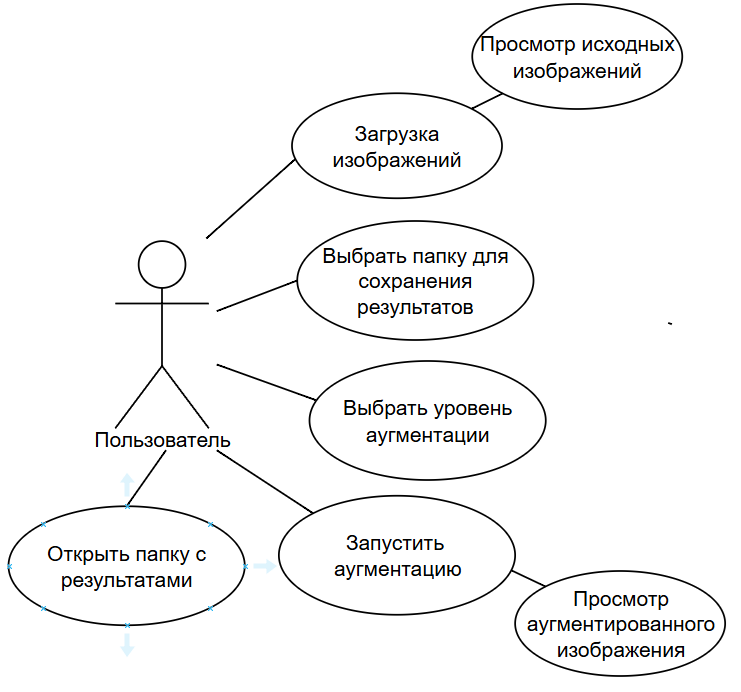
\includegraphics[width=0.7\linewidth]{images/diagrampreced}
	\caption{Диаграмма прецедентов}
	\label{fig:diagrampreced}
\end{figure}


\paragraph{Вариант использования «Загрузка изображений»}

Заинтересованные лица и их требования:
Пользователь желает загрузить изображения из локальной папки для дальнейшей обработки.
Предусловие:
Программа запущена, главное окно отображается.
Постусловие:
Список изображений успешно загружен и готов к обработке. Отображается предварительный просмотр одного изображения.
Основной успешный сценарий:
\begin{enumerate}
	\item Пользователь нажимает кнопку «Загрузить папку».
	\item Открывается стандартный диалог выбора папки.
	\item Пользователь выбирает папку, содержащую изображения.
	\item Программа считывает все подходящие файлы по расширениям (.jpg, .jpeg, .png, .bmp).
	\item Если изображения найдены — отображается их количество и предварительный просмотр одного изображения.
	\item Если изображения отсутствуют — отображается предупреждение.
\end{enumerate}

\paragraph{Вариант использования «Выбор папки для сохранения»}

Заинтересованные лица и их требования:
Пользователь хочет указать папку, куда будут сохранены результаты аугментации.
Предусловие:
Программа запущена. Загружены изображения.
Постусловие:
Путь для сохранения результатов успешно сохранён и отображается в интерфейсе.
Основной успешный сценарий:

\begin{enumerate}
	\item Пользователь нажимает кнопку «Выбрать папку для сохранения».
	\item Открывается стандартный диалог выбора папки.
	\item Пользователь выбирает папку.
	\item Путь к папке отображается в информационном блоке программы.
\end{enumerate}

\paragraph{Вариант использования «Выбор уровня аугментации»}

Заинтересованные лица и их требования:
Пользователь хочет определить интенсивность применяемых преобразований к изображениям.
Предусловие:
Программа запущена, изображения загружены.
Постусловие:
Уровень аугментации (low, medium, high) выбран и сохранён до момента применения обработки.
Основной успешный сценарий:

\begin{enumerate}
	\item Пользователь нажимает на выпадающий список.
	\item Пользователь выбирает один из доступных уровней.
	\item Программа сохраняет выбранный уровень для дальнейшей обработки.
\end{enumerate}

\paragraph{Вариант использования «Применение аугментации»}

Заинтересованные лица и их требования:
Пользователь хочет обработать загруженные изображения с применением выбранных методов.
Предусловие:
Загружены изображения, выбран уровень аугментации и папка для сохранения.
Постусловие:
Аугментированные изображения сохранены в выбранную папку. Отображается сообщение об успешном завершении.
Основной успешный сценарий:

\begin{enumerate}
	\item Пользователь нажимает кнопку «Применить аугментацию».
	\item Программа проверяет, загружены ли изображения и выбрана ли папка.
	\item Каждое изображение предварительно масштабируется и передаётся в модуль обработки.
	\item Модуль обработки применяет выбранные аугментации.
	\item Результаты сохраняются с модифицированными именами в выбранной папке.
	\item Программа отображает сообщение об успешной обработке.
\end{enumerate}

\paragraph{Вариант использования «Предпросмотр изображений»}

Заинтересованные лица и их требования:
Пользователь хочет увидеть исходное изображение и результат аугментации для визуальной оценки.
Предусловие:
Изображения загружены, аугментация завершена.
Постусловие:
В интерфейсе отображается пара: оригинал и результат аугментации.
Основной успешный сценарий:

\begin{enumerate}
	\item После завершения аугментации, программа отображает исходное изображение и один из полученных результатов.
	\item Пользователь визуально оценивает результат на встроенных миниатюрах (QLabel).
\end{enumerate}

\paragraph{Вариант использования «Предпросмотр изображений до и после»}

Заинтересованные лица и их требования:
Пользователь хочет визуально сравнить исходное изображение и результат аугментации.
Предусловие:
Минимум одно изображение успешно обработано. В интерфейсе доступна панель предпросмотра.
Постусловие:
На экране отображаются миниатюры: исходное и аугментированное изображение. Пользователь может переходить к следующей паре.
Основной успешный сценарий:

\begin{enumerate}
	\item После завершения аугментации, интерфейс отображает первое изображение до обработки и один из его аугментированных вариантов.
	\item Под предпросмотром расположены кнопки: «Предыдущее», «Следующее».
	\item При нажатии на «Следующее», отображается следующая пара (оригинал и результат).
	\item Если достигнут конец списка, кнопка «Следующее» становится недоступной.
	\item Аналогично работает кнопка «Предыдущее».
\end{enumerate}

\paragraph{Вариант использования «Открытие папки с аугментированными изображениями»}

Заинтересованные лица и их требования:
Пользователь хочет быстро открыть в проводнике папку с готовыми результатами.
Предусловие:
Папка для сохранения результатов была выбрана, аугментация успешно завершена.
Постусловие:
Открывается системный файловый менеджер в выбранной ранее директории.
Основной успешный сценарий:
\begin{enumerate}
	\item Пользователь нажимает кнопку «Открыть папку с результатами».
	\item Программа проверяет наличие валидного пути к папке.
	\item Если путь существует, открывается стандартный проводник (используется QDesktopServices.openUrl()).
	\item Если путь не был указан или папка недоступна, появляется сообщение об ошибке.
\end{enumerate}

\subsection{Вариант использования «Загрузка изображений»}

Разработка программной документации и программного изделия должна производиться согласно ГОСТ 19.102-77 и ГОСТ 34.601-90. Единая система программной документации.

Программная документация должна включать в себя:
\begin{itemize}
	\item анализ предметной области;
	\item техническое задание;
	\item технический проект;
	\item рабочий проект.
\end{itemize}

\section{Технический проект}
\subsection{Общая характеристика организации решения задачи}

Необходимо спроектировать и разработать сайт, который должен способствовать продвижению компании на рынке.
Основной задачей системы является автоматизированная обработка изображений, загруженных пользователем из выбранной директории, с последующим применением набора предопределённых преобразований (аугментаций) и сохранением полученных результатов в отдельную директорию. Пользователь должен иметь возможность выбрать уровень интенсивности аугментации (низкий, средний, высокий), задать папку для сохранения и просматривать результаты преобразования в виде предварительного просмотра.
Обработка изображений осуществляется на стороне клиента, без необходимости подключения к сети Интернет. Это позволяет обеспечить максимальную независимость и приватность данных. Программа ориентирована на стабильную работу в среде Windows/Linux с минимальными системными требованиями и без фоновых сетевых процессов.

\subsection{Обоснование выбора технологий проектирования}

Используемые при разработке технологии отвечают современным стандартам и обеспечивают надёжность, удобство сопровождения и масштабируемость проекта. Для построения графического интерфейса выбрана кросс-платформенная библиотека PySide6, а для работы с изображениями — проверенная временем библиотека Pillow.

\subsubsection{Язык программирования Python}

Язык программирования Python был выбран как основной инструмент для реализации системы в силу следующих причин:

\begin{itemize}
	\item простота синтаксиса, позволяющая ускорить этапы разработки и отладки;
	\item широкая экосистема библиотек, включая Pillow для работы с изображениями и PySide6 для построения графического интерфейса;
	\item хорошая читаемость и расширяемость кода, что важно для последующего сопровождения проекта или его масштабирования;
	\item поддержка мультиплатформенности: программа может быть развёрнута как на Windows, так и на Linux, без необходимости значительных изменений в коде;
	\item активное сообщество и постоянное развитие языка и его инструментов.
\end{itemize}

Python используется как для создания пользовательского интерфейса, так и для реализации логики обработки изображений, что позволяет обеспечить целостность архитектуры и снизить сложность сопровождения программной системы.

\subsubsection{Исследование и выбор методов аугментации изображений}

Аугментация изображений (image augmentation) представляет собой процесс искусственного увеличения объема обучающей выборки путём внесения различных преобразований в исходные изображения. Актуальность применения аугментации особенно высока при работе с ограниченным числом изображений, в том числе для задач классификации, детекции и сегментации.

Цели внедрения аугментации в рамках настоящего программного решения:

\begin{itemize}
	\item увеличение разнообразия обучающей выборки без реального увеличения числа изображений;
	\item снижение переобучения алгоритмов машинного обучения при последующем применении данных;
	\item имитирование реальных условий съёмки, включая различия в освещении, положении камеры, шумовых помехах и т.д.;
	\item тестирование устойчивости алгоритмов распознавания и аналитики к искажениям;
	\item поддержка регуляризации и улучшение обобщающей способности обучаемых моделей.
\end{itemize}

%РИСУНОК
%Изображение сетка 2×3: оригинал и пять результатов (rotate, flip, noise, brightness, shift). 

Процесс отбора подходящих методов аугментации был организован в несколько этапов:

\begin{enumerate}
	\item Анализ имеющихся методов аугментации, реализуемых через библиотеки PIL, OpenCV и imgaug. Рассматривались следующие трансформации: геометрические (повороты, масштабирование, сдвиги, отражения), композиционные (обрезка, наложение).
	\item Формирование предварительного пула методов: поворот, шум (гауссовский, «соль и перец»), отражение, сдвиг, изменение яркости, обрезка, изменение контрастности.
	\item Применение методов к тестовой выборке (около 100 изображений), анализ визуальных изменений, а также оценка влияния на читаемость структуры изображения.
	\item Формализация критериев отбора: сохранение семантики изображения (разборчивость объектов), воспроизводимость и параметризация, реальная применимость к задачам распознавания и визуального анализа.
	\item Исключение методов, создающих риск искажения семантики (например, scale и агрессивный crop) или плохо применимых в условиях ограниченных вычислительных ресурсов.
\end{enumerate}

%таблица с видами аугментации

Таким образом, отбор прошли пять ключевых методов, которые соответствуют критериям качества, скорости и реалистичности: rotate, noise, flip, shift, brightness.

\subsubsection{Описание и исследование выбранных методов аугментации}

Для достижения наилучшего эффекта преобразования изображений были выбраны пять методов. В данном разделе проводится их подробный анализ, в том числе: принцип работы, исследованные диапазоны параметров, визуальные результаты и рекомендации по применению.

\begin{enumerate}
	\item Поворот изображения.

Поворот изображения на определённый угол позволяет имитировать изменение положения камеры или объекта. Преобразование сохраняет геометрию объектов и является одним из наименее деструктивных способов аугментации.

Пусть изображение задано в виде двемерной матрицы I(x, y) где, x, y принадлежит Z - координаты пикселей. Поворот изображения на угол в радианах вокруг центра ($x_c$, $y_c$) осуществляется по следующим формулам:


\[
\begin{bmatrix}
	x' \\
	y'
\end{bmatrix}
=
\begin{bmatrix}
	\cos\theta & -\sin\theta \\
	\sin\theta & \cos\theta
\end{bmatrix}
\cdot
\begin{bmatrix}
	x - x_c \\
	y - y_c
\end{bmatrix}
+
\begin{bmatrix}
	x_c \\
	y_c
\end{bmatrix}
\]

где $(x', y')$ — новые координаты пикселя после поворота. Угол $\theta$ считается положительным при повороте против часовой стрелки.

Диапазон параметров:
\begin{itemize}
	\item углы поворота: от -25 до +25 градусов;
	\item шаг исследуемых значений: 5 градусов.
\end{itemize}

Углы выше 30° приводят к искажению восприятия, особенно при наличии симметричных объектов. Было установлено, что диапазон ±25° обеспечивает визуальное разнообразие без потери информативности.

%ИЗОБРАЖЕНИЕ И ВАРИАНТЫ ПОВОРОТА -15 0 И 15 ГРАДУСОВ

	\item Добавление шума.
	
Добавление шумов позволяет имитировать условия плохой съёмки, передаёт реалистичность восприятия, особенно для задач, где необходимо устойчивое поведение к зашумлённым данным. Рассматривались два типа: гауссовский шум и соль и перец.

Гауссовский шум описывается добавлением случайной величины, распределённой по нормальному закону:

\[
I'(x, y) = I(x, y) + \mathcal{N}(0, \sigma^2),
\]
где $\mathcal{N}(0, \sigma^2)$ — нормально распределённая случайная величина со средним $0$ и дисперсией $\sigma^2$. Все значения выходного изображения ограничиваются диапазоном допустимых значений яркости (например, $[0, 255]$).
	
Шум типа «соль и перец» реализуется случайной заменой значения пикселей на минимальное (чёрное) или максимальное (белое) значение с заданной вероятностью $p$:

\[
I'(x, y) =
\begin{cases}
	0, & \text{с вероятностью } p/2 \\
	255, & \text{с вероятностью } p/2 \\
	I(x, y), & \text{с вероятностью } 1 - p
\end{cases}
\]


Диапазон параметров:
\begin{itemize}
	\item среднеквадратичное отклонение (гауссов шум): 2-25;
	\item соль и перец(процент испорченных пикселей): 0.01 - 0.10 (1-10\%).
\end{itemize}

При превышении указанных значений изображение становится трудноузнаваемым. Оптимальные значения были выбраны методом экспертной оценки и визуального тестирования.

%ИЗБОБРАЖЕНИЕ
% Примеры зашумления изображений с разной интенсивностью

	\item Отражение.
	
Отражение изображения по горизонтали или вертикали. Простой способ создания новых примеров без искажения формы. Отражение изображения по горизонтали или вертикали — это простая перестановка координат пикселей.


Горизонтальное отражение:

\[
I'(x, y) = I(W - 1 - x, y)
\]

где $W$ — ширина изображения.
	
Вертикальное отражение:

\[
I'(x, y) = I(x, H - 1 - y)
\]

где $H$ — высота изображения.


Обычно используется только горизонтальное отражение, так как вертикальное может нарушить семантику изображения (например, перевёрнутый текст или искажение направления объектов). 

%ИЗОБРАЖЕНИЕ оригинал и отраженное изображение

	\item Сдвиг.

Сдвиг изображения по горизонтали и вертикали, позволяющий сместить объект в пределах кадра, не нарушая общей структуры. 
Сдвиг изображения — это перемещение пикселей вдоль осей $X$ и/или $Y$ на заданное количество пикселей $\Delta x$ и $\Delta y$. При выходе за границы изображения пустые области заполняются фоновым значением (например, чёрным — 0).

\[
I'(x, y) =
\begin{cases}
	I(x - \Delta x, y - \Delta y), & \text{если } (x - \Delta x, y - \Delta y) \in \text{область изображения} \\
	0, & \text{иначе}
\end{cases}
\]

Сдвиги задаются как процент от размеров изображения:
\[
\Delta x = \alpha_x \cdot W,\quad \Delta y = \alpha_y \cdot H,\quad \alpha_x, \alpha_y \in [-0.15, 0.15]
\]

Диапазон параметров:

Смещение по X и Y: от -15\% до +15\% от размера изображения

Смещения более чем на 20\% влекут за собой обрезку ключевых областей. Оптимальные значения позволяют сохранить композицию при создании новой геометрии расположения объектов.

%ИЗОБРАЖЕНИЕ
%смещение по горзонтали +-10%


	\item Изменение яркости.

Изменение яркости изображения имитирует освещение в различных условиях (день, ночь, контровой свет и т.п.). Это особенно важно для универсализации восприятия моделей. Оно предполагает умножение значений всех пикселей изображения на коэффициент $\gamma \in [0.6, 1.4]$, где:

\begin{itemize}
	\item $\gamma < 1$ — затемнение изображения;
	\item $\gamma > 1$ — увеличение яркости.
\end{itemize}

\[
I'(x, y) = \text{clip}\left( \gamma \cdot I(x, y),\ 0,\ 255 \right)
\]

Диапазон параметров: коэффициент изменения яркости: 0.6 – 1.4
(где 1.0 — исходное значение)

Значения ниже 0.5 делают изображение почти чёрным, выше 1.5 — засвеченным. Оптимальный диапазон обеспечивает баланс между реализмом и информативностью.

% ИЗОБРАЖЕНИЕ
% зимененение яркости 0.6, 1.0, 1.4

\end{enumerate}

%таблица выбранных оптимальных значений

\subsubsection{Конфигурация уровней аугментации и автоматизация параметров}

Для повышения гибкости и упрощения взаимодействия с системой аугментации в пользовательском интерфейсе были реализованы три уровня интенсивности преобразований: low, medium и high. Каждый уровень соответствует предопределённому набору параметров, автоматически применяемых к каждому изображению.

\textbf{Обоснование уровней}

Уровни были выделены на основе эмпирического анализа, где оценивалась степень трансформации и её влияние на восприятие изображения. % На таблице ниже представлены сводные настройки для каждого уровня
\begin{itemize}
	\item low - отражение, яркость;
	\item medium - отражение, яркость, поворот, шум;
	\item high - отражение, яркость, поворот, шум, сдвиг.
\end{itemize}
	
%ИЗОБРАЖЕНИЕ
%Сравнение изображений при применении уровней low, medium, high.

Система построена по принципу передачи параметров через уровень аугментации. Пользователь выбирает нужный уровень в интерфейсе, и далее программа сопоставляет уровень с конфигурацией (словарь параметров), применяет соответствующие методы аугментации, обеспечивает единообразное поведение для всех изображений партии. Выделение уровней аугментации: упрощает пользовательский опыт, обеспечивает стабильность качества результатов и позволяет масштабировать систему без изменений в логике преобразований.

Для обоснования применимости выбранных методов аугментации и их параметров была проведена оценка качества сгенерированных изображений по следующим критериям:
\begin{itemize}
	\item визуальная читаемость изображения (отсутствие чрезмерных искажений);
	\item сохранение признаков исходного объекта (не теряются ключевые контуры, формы, текстуры);
	\item разнообразие выборки (каждая аугментация должна вносить полезную вариативность, а не избыточный шум);
	\item устойчивость к переобучению на основе опыта использования в системах распознавания (принцип увеличения генерализации).
\end{itemize}

На основании анализа параметров можно выделить следующие оптимальные значения:

\begin{itemize}
	\item поворот: +-15 градусов (максимум 25 градусов);
	\item гауссов шум: 10-15;
	\item соль/Перец: 3-5\%;
	\item яркость: от 0.8 до 1.2;
	\item до 10\% по X и Y;
	\item горизонтальное.
\end{itemize}

\ifПрактика{}\else{
   \section{Рабочий проект}
\subsection{Спецификация компонентов и классов программы}

\subsection{Модуль shift.py}

Модуль shift.py содержит функцию для случайного сдвига изображения по осям X и Y. Модуль не содержит классов. Метод модуля - shift image. Он выполняет случайный сдвиг изображения на расстояние, не превышающее заданный процент от его размеров, с использованием аффинного преобразования. Входные данные:

\begin{itemize}
	\item image (тип PIL.Image.Image) – исходное изображение для сдвига;
	\item max shift (тип float, значение по умолчанию = 0.1) – максимальный процент сдвига от размера изображения.
\end{itemize}

Возвращаемые данные: PIL.Image.Image – изображение после сдвига.

\subsection{Модуль brightness.py}

Модуль brightness.py предоставляет функцию для изменения яркости изображения. Модуль не содержит классов. Метод модуля - change brightness. Он изменяет яркость изображения с использованием класса ImageEnhance.Brightness из библиотеки Pillow. Входные данные:

\begin{itemize}
	\item image (тип PIL.Image.Image) – исходное изображение;
	\item factor (тип float, значение по умолчанию = 1.0) – коэффициент яркости (меньше 1 – затемнение, больше 1 – осветление).
\end{itemize}

Возвращаемые данные: PIL.Image.Image – изображение с измененной яркостью.

\subsection{Модуль rotate.py}

Модуль rotate.py содержит функцию для поворота изображения на заданный угол. Модуль не содержит классов. Метод модуля - rotate image. Он выполняет поворот изображения на заданный угол с возможностью изменения размера после поворота. Входные данные:

\begin{itemize}
	\item image (тип PIL.Image.Image) – исходное изображение;
	\item angle (тип float) – угол поворота в градусах;
	\item target size (тип tuple, необязательный) – целевой размер изображения после поворота (ширина, высота).
\end{itemize}

Возвращаемые данные: PIL.Image.Image – повернутое изображение (и измененного размера, если указан target size).

\subsection{Модуль flip.py}

Модуль flip.py предоставляет функцию для отражения изображения по горизонтали или вертикали. Модуль не содержит классов. Метод модуля - flip image. Он отражает изображение по горизонтали или вертикали с использованием метода transpose из библиотеки Pillow. При некорректном значении параметра mode вызывает исключение ValueError. Входные данные:

\begin{itemize}
	\item image (тип PIL.Image.Image) – исходное изображение;
	\item mode (тип str, значение по умолчанию = 'horizontal') – режим отражения (horizontal или vertical).
\end{itemize}

Возвращаемые данные: PIL.Image.Image – отраженное изображение.

\subsection{Модуль noise.py}

Модуль noise.py содержит функцию для добавления шума к изображению в градациях серого. Модуль не содержит классов. Метод модуля - add noise. Он добавляет к изображению шум типа "гауссовский" или "соль и перец". Для обработки используется библиотека NumPy. Требует, чтобы изображение было в режиме L, иначе вызывает исключение ValueError. Входные данные:

\begin{itemize}
	\item image (тип PIL.Image.Image) – исходное изображение в режиме L (градации серого);
	\item noise type (тип str, значение по умолчанию = 'gaussian') – тип шума (gaussian или salt pepper);
	\item **kwargs – дополнительные параметры:
	\begin{itemize}
		\item для gaussian: stddev (тип float, значение по умолчанию = 10) – стандартное отклонение шума;
		\item для salt pepper: amount (тип float, значение по умолчанию = 0.05) – доля пикселей, затронутых шумом; salt vs pepper (тип float, значение по умолчанию = 0.5) – соотношение "соли" и "перца".
	\end{itemize}
\end{itemize}

Возвращаемые данные: PIL.Image.Image – изображение с добавленным шумом.

\subsection{Модуль augmentation config.py}

Модуль augmentation config.py определяет конфигурацию аугментаций. Модуль не содержит классов или методов, представляя собой словарь augmentation config. Описание конфигурации:

\begin{itemize}
	\item available augmentations (тип list) – список доступных аугментаций: noise, rotate, flip, shift, brightness;
	\item noise, rotate, flip, shift, brightness (тип dict) – настройки для каждой аугментации с полями enabled и params (например, angle range, std range);
	\item volume presets (тип dict) – предустановленные объемы генерации: 1х25, 1х50, 1х100.
\end{itemize}

Он обеспечивает централизованное управление параметрами аугментаций и их состоянием.

\subsection{Модуль pipeline.py}

Модуль pipeline.py реализует логику применения аугментаций. Он обеспечивает централизованное управление параметрами аугментаций и их состоянием. Методы модуля представлены в таблице ~\ref{table:pipeline}.

\renewcommand{\arraystretch}{0.8} % уменьшение расстояний до сетки таблицы
\begin{xltabular}{\textwidth}{|X|X|X|X|X|}
	\caption{Методы модуля pipeline.py\label{table:pipeline}}\\
	\hline 
	\centrow \setlength{\baselineskip}{0.7\baselineskip} Название метода & 
	\centrow Параметры метода &
	\centrow Возвращаемое значение & 
	\centrow Назначение метода \\ 
	\hline 
	\endfirsthead
	
	\caption*{Продолжение таблицы \ref{table:pipeline}}\\
	\hline 
	\centrow Название метода & 
	\centrow Параметры метода &
	\centrow Возвращаемое значение & 
	\centrow Назначение метода \\ 
	\hline 
	\endhead
	
	\_\_init\_\_ & Не имеет & Не имеет  & Инициализирует главное окно программы, задает его параметры, заголовок, панель меню с действиями для переключения режимов. \\ \hline 
	
	apply\_ augmentation & image (тип PIL.Image. Image) – изображение; augmentation\_ type (тип str) – тип аугментации & PIL.Image. Image – аугментированное изображение & Применяет одну аугментацию в соответствии с конфигурацией.\\
	\hline
	
	process\_ images & image (тип PIL.Image. Image) – изображение; target\_size (тип tuple) – размер; volume\_level (тип str, по умолчанию 'low') – уровень генерации & list – список аугментированных изображений & Генерирует заданное количество аугментированных версий с случайными комбинациями аугментаций.\\
	\hline
	
	process\_ images & image (тип PIL.Image. Image) – изображение; target\_size (тип tuple) – размер; volume\_level (тип str, по умолчанию 'low') – уровень генерации & list – список аугментированных изображений & Генерирует заданное количество аугментированных версий с случайными комбинациями аугментаций.\\
	\hline
	
\end{xltabular}
\renewcommand{\arraystretch}{1.0} % восстановление сетки
\vspace{-\baselineskip}


\subsection{Модуль main\_window.py}

Модуль main\_window предоставляет графический интерфейс для взаимодействия с пользователем, включая загрузку изображений, выбор директории, настройку аугментаций, предпросмотр и сохранение результатов. Константы и методы: отсутствуют.

Класс MainWindow (модуль main\_window.py).

Базовый класс: AugmentationWindow (из модуля ui.window).

Внутренние поля представлены в таблице ~\ref{table:main_window}.

\begin{xltabular}{\textwidth}{|X|X|X|}
	\caption{Внутренние поля класса MainWindow \label{table:main_window}} \\
	\hline 
	\centrow Внутреннее поле & 
	\centrow Тип & 
	\centrow Описание \\ 
	\hline 
	\endfirsthead
	
	\caption*{Продолжение таблицы \ref{table:main_window}} \\
	\hline 
	\centrow Внутреннее поле & 
	\centrow Тип & 
	\centrow Описание \\ 
	\hline 
	\endhead
	
	output\_dir & str или None & Путь к директории для сохранения результатов. \\ \hline
	image\_paths & list & Список путей к загруженным изображениям. \\ \hline
	progress\_bar & QProgressBar & Виджет для отображения прогресса обработки. \\ \hline
	scroll\_area & QScrollArea & Область прокрутки для отображения миниатюр. \\ \hline
	preview\_container & QWidget & Контейнер для размещения миниатюр аугментированных изображений. \\ \hline
	preview\_layout & QHBoxLayout & Макет для размещения миниатюр. \\ \hline
	select\_augs\_button & QPushButton & Кнопка для открытия диалога выбора аугментаций. \\ \hline
\end{xltabular}

Методы класса представлены в таблице ~\ref{table:main_window_method}.

\renewcommand{\arraystretch}{0.8} % уменьшение расстояний до сетки таблицы
\begin{xltabular}{\textwidth}{|X|X|X|X|X|}
	\caption{Методы модуля pipeline.py\label{table:main_window_method}}\\
	\hline 
	\centrow \setlength{\baselineskip}{0.7\baselineskip} Название метода & 
	\centrow Параметры метода &
	\centrow Возвращаемое значение & 
	\centrow Назначение метода \\ 
	\hline 
	\endfirsthead
	
	\caption*{Продолжение таблицы \ref{table:main_window_method}}\\
	\hline 
	\centrow Название метода & 
	\centrow Параметры метода &
	\centrow Возвращаемое значение & 
	\centrow Назначение метода \\ 
	\hline 
	\endhead
	
	load\_images & Не имеет & Не имеет  & Загружает изображения из выбранной папки и отображает предпросмотр первого. \\ \hline
	
	select\_output \_folder & Не имеет & Не имеет  & Загружает изображения из выбранной папки и отображает предпросмотр первого. \\ \hline

	open\_output\_ directory & Не имеет & Не имеет  & Открывает папку с результатами в файловом менеджере. \\ \hline 

	show\_image \_preview & path (тип str) – путь к изображению & Не имеет  & Отображает предпросмотр исходного изображения в интерфейсе. \\ \hline 

	show\_ augmented\_ preview & pil\_image (тип PIL.Image.Image) – аугментированное изображение & Не имеет & Отображает предпросмотр аугментированного изображения в интерфейсе. \\ \hline
	
	apply\_ selected\_ augmentation & Не имеет & Не имеет & Выполняет аугментацию для всех загруженных изображений и сохраняет результаты. \\ \hline
	
	open\_ augmentation \_selector & Не имеет & Не имеет & Открывает диалог для настройки активных аугментаций. \\ \hline
	
	apply\_ augmentation & image (тип PIL.Image. Image) – изображение; augmentation\_ type (тип str) – тип аугментации & PIL.Image. Image – аугментированное изображение & Применяет одну аугментацию в соответствии с конфигурацией.\\
	\hline
	
	process\_ images & image (тип PIL.Image. Image) – изображение; target\_size (тип tuple) – размер; volume\_level (тип str, по умолчанию 'low') – уровень генерации & list – список аугментированных изображений & Генерирует заданное количество аугментированных версий с случайными комбинациями аугментаций.\\
	\hline
	
	process\_ images & image (тип PIL.Image. Image) – изображение; target\_size (тип tuple) – размер; volume\_level (тип str, по умолчанию 'low') – уровень генерации & list – список аугментированных изображений & Генерирует заданное количество аугментированных версий с случайными комбинациями аугментаций.\\
	\hline
	
\end{xltabular}
\renewcommand{\arraystretch}{1.0} % восстановление сетки
\vspace{-\baselineskip}

\subsection{Модуль augmentation\_selector.py}

Модуль augmentation\_selector.py предоставляет диалоговое окно для выбора активных аугментаций. Константы: отсутствуют. Метод get\_selected\_augmentations возвращает список аугментаций, отмеченных пользователем.

Внутренние поля представлены в таблице ~\ref{table:augmentation_selector}.

\begin{xltabular}{\textwidth}{|X|X|X|}
	\caption{Внутренние поля класса MainWindow \label{table:augmentation_selector}} \\
	\hline 
	\centrow Внутреннее поле & 
	\centrow Тип & 
	\centrow Описание \\ 
	\hline 
	\endfirsthead
	
	\caption*{Продолжение таблицы \ref{table:main_window}} \\
	\hline 
	\centrow Внутреннее поле & 
	\centrow Тип & 
	\centrow Описание \\ 
	\hline 
	\endhead
	
	selected & set & Множество выбранных пользователем аугментаций. \\ \hline
	checkboxes & dict & Словарь, где ключ – название аугментации, значение – QCheckBox. \\ \hline
\end{xltabular}

\subsection{Модульное тестирование разработанной программной системы}.

Модульное тестирование проведено для проверки корректности работы отдельных компонентов программной системы аугментации изображений. Тестирование осуществлялось с использованием библиотеки unittest языка Python, что позволило автоматизировать проверки функциональности функций и классов. Для каждого модуля сформированы таблицы тестовых наборов, содержащие описание теста, входные данные и эталонные выходные данные. Тесты выполнялись на тестовом изображении размером $100 \times 100$ пикселей, созданном программно с использованием библиотеки Pillow. Все тесты успешно пройдены, что подтверждает отсутствие ошибок в реализованных компонентах.

\subsubsection{Тестовые наборы для модуля shift.py}

Тестовые наборы для модуля shift.py представлены в таблице ~\ref{tab:test_shift}.

\begin{xltabular}{\textwidth}{|X|X|X|}
	\caption{Тестовые наборы для функции shift\_image (shift.py) \label{tab:test_shift}} \\
	\hline
	\centrow Описание теста &
	\centrow Входные данные &
	\centrow Эталонные выходные данные \\
	\hline
	\endfirsthead
	
	\caption*{Продолжение таблицы \ref{tab:test_shift}} \\
	\hline
	\centrow Описание теста &
	\centrow Входные данные &
	\centrow Эталонные выходные данные \\
	\hline
	\endhead
	
	Проверка корректного сдвига изображения на 10 \% по горизонтали. & Изображение $100 \times 100$ пикселей, max\_shift=0.1, фиксированный сдвиг 10 пикселей. & Изображение $100 \times 100$ пикселей с сдвигом на 10 пикселей, заполнение пустых областей белым цветом. \\ \hline
	Проверка отсутствия изменения размеров при сдвиге. & Изображение $100 \times 100$ пикселей, max\_shift=0.05, случайный сдвиг. & Изображение $100 \times 100$ пикселей, без изменения размеров. \\ \hline
\end{xltabular}

\subsubsection{Тестовые наборы для модуля brightness.py}

Тестовые наборы для модуля brightness.py представлены в таблице ~\ref{tab:test_brightness}.


\begin{xltabular}{\textwidth}{|X|X|X|}
	\caption{Тестовые наборы для функции change\_brightness (brightness.py) \label{tab:test_brightness}} \\
	\hline
	\centrow Описание теста &
	\centrow Входные данные &
	\centrow Эталонные выходные данные \\
	\hline
	\endfirsthead
	
	\caption*{Продолжение таблицы \ref{tab:test_brightness}} \\
	\hline
	\centrow Описание теста &
	\centrow Входные данные &
	\centrow Эталонные выходные данные \\
	\hline
	\endhead
	
	Проверка увеличения яркости на 50 \%. & Изображение $100 \times 100$ пикселей с серым цветом (128, 128, 128), factor=1.5. & Изображение $100 \times 100$ пикселей с увеличенной яркостью (192, 192, 192). \\ \hline
	Проверка сохранения исходной яркости при factor=1.0. & Изображение $100 \times 100$ пикселей с цветом (100, 100, 100), factor=1.0. & Изображение $100 \times 100$ пикселей с сохраненными значениями (100, 100, 100). \\ \hline
\end{xltabular}

\subsubsection{Тестовые наборы для модуля rotate.py}

Тестовые наборы для модуля rotate.py представлены в таблице ~\ref{tab:test_rotate}.

\begin{xltabular}{\textwidth}{|X|X|X|}
	\caption{Тестовые наборы для функции rotate\_image (rotate.py) \label{tab:test_rotate}} \\
	\hline
	\centrow Описание теста &
	\centrow Входные данные &
	\centrow Эталонные выходные данные \\
	\hline
	\endfirsthead
	
	\caption*{Продолжение таблицы \ref{tab:test_rotate}} \\
	\hline
	\centrow Описание теста &
	\centrow Входные данные &
	\centrow Эталонные выходные данные \\
	\hline
	\endhead
	
	Проверка поворота на 90 градусов с сохранением размера. & Изображение $100 \times 100$ пикселей, angle=90, target\_size=(100, 100). & Изображение $100 \times 100$ пикселей, повернутое на 90 градусов. \\ \hline
	Проверка корректного заполнения при повороте на 45 градусов & Изображение $100 \times 100$ пикселей, angle=45, target\_size=(100, 100). & Изображение $100 \times 100$ пикселей с поворотом на 45 градусов и заполнением белым цветом. \\ \hline
\end{xltabular}

\subsubsection{Тестовые наборы для модуля flip.py}

Тестовые наборы для модуля flip.py представлены в таблице ~\ref{tab:test_flip}.

\begin{xltabular}{\textwidth}{|X|X|X|}
	\caption{Тестовые наборы для функции flip\_image (flip.py) \label{tab:test_flip}} \\
	\hline
	\centrow Описание теста &
	\centrow Входные данные &
	\centrow Эталонные выходные данные \\
	\hline
	\endfirsthead
	
	\caption*{Продолжение таблицы \ref{tab:test_flip}} \\
	\hline
	\centrow Описание теста &
	\centrow Входные данные &
	\centrow Эталонные выходные данные \\
	\hline
	\endhead
	
	Проверка горизонтального отражения. & Изображение $100 \times 100$ пикселей с градиентом слева направо. & Изображение $100 \times 100$ пикселей с зеркальным отражением градиента. \\ \hline
	Проверка вертикального отражения. & Изображение $100 \times 100$ пикселей с градиентом сверху вниз. & Изображение $100 \times 100$ пикселей с вертикальным отражением градиента. \\ \hline
\end{xltabular}

\subsubsection{Тестовые наборы для модуля noise.py}

Тестовые наборы для модуля noise.py представлены в таблице ~\ref{tab:test_noise}.

\begin{xltabular}{\textwidth}{|X|X|X|}
	\caption{Тестовые наборы для функции add\_noise (noise.py) \label{tab:test_noise}} \\
	\hline
	\centrow Описание теста &
	\centrow Входные данные &
	\centrow Эталонные выходные данные \\
	\hline
	\endfirsthead
	
	\caption*{Продолжение таблицы \ref{tab:test_noise}} \\
	\hline
	\centrow Описание теста &
	\centrow Входные данные &
	\centrow Эталонные выходные данные \\
	\hline
	\endhead
	
	Проверка добавления гауссовского шума. & Изображение $100 \times 100$ пикселей в градациях серого, stddev=10. & Изображение $100 \times 100$ пикселей с добавленным гауссовским шумом, дисперсия увеличена. \\ \hline
	Проверка шума "соль и перец" с долей 5 \%. & Изображение $100 \times 100$ пикселей, noise\_type='salt\_pepper', amount=0.05. & Изображение $100 \times 100$ пикселей с 5 \% пикселей заменено на черный или белый цвет. \\ \hline
\end{xltabular}

\subsubsection{Тестовые наборы для модуля pipeline.py}

Тестовые наборы для модуля pipeline.py представлены в таблице ~\ref{tab:test_pipeline}.

\begin{xltabular}{\textwidth}{|X|X|X|}
	\caption{Тестовые наборы для функции process\_images (pipeline.py) \label{tab:test_pipeline}} \\
	\hline
	\centrow Описание теста &
	\centrow Входные данные &
	\centrow Эталонные выходные данные \\
	\hline
	\endfirsthead
	
	\caption*{Продолжение таблицы \ref{tab:test_pipeline}} \\
	\hline
	\centrow Описание теста &
	\centrow Входные данные &
	\centrow Эталонные выходные данные \\
	\hline
	\endhead
	
	Проверка генерации 3 аугментированных изображений. & Изображение $100 \times 100$ пикселей, volume\_level='1х25' с изменением на 3. & Список из 3 аугментированных изображений размером $100 \times 100$ пикселей. \\ \hline
	Проверка корректности именования файлов. & Изображение $100 \times 100$ пикселей, volume\_level='1х25', сохранение в папку. & Файлы с именами вроде test\_aug\_001.png, test\_aug\_002.png, test\_aug\_003.png. \\ \hline
\end{xltabular}

\subsubsection{Тестовые наборы для модуля main\_window.py}

Тестовые наборы для модуля main\_window.py представлены в таблице ~\ref{tab:test_main_window}.

\begin{xltabular}{\textwidth}{|X|X|X|}
	\caption{Тестовые наборы для класса MainWindow (main\_window.py) \label{tab:test_main_window}} \\
	\hline
	\centrow Описание теста &
	\centrow Входные данные &
	\centrow Эталонные выходные данные \\
	\hline
	\endfirsthead
	
	\caption*{Продолжение таблицы \ref{tab:test_main_window}} \\
	\hline
	\centrow Описание теста &
	\centrow Входные данные &
	\centrow Эталонные выходные данные \\
	\hline
	\endhead
	
	Проверка загрузки одного изображения. & Папка с одним изображением $100 \times 100$ пикселей. & image\_count = 1, отображение предпросмотра. \\ \hline
	Проверка загрузки нескольких изображений. & Папка с тремя изображениями $100 \times 100$ пикселей. & image\_count = 3, отображение списка предпросмотров. \\ \hline
\end{xltabular}

\subsubsection{Тестовые наборы для модуля augmentation\_selector.py}

Тестовые наборы для модуля augmentation\_selector.py представлены в таблице ~\ref{tab:test_augmentation_selector}.

\begin{xltabular}{\textwidth}{|X|X|X|}
	\caption{Тестовые наборы для класса AugmentationSelectorDialog (augmentation\_selector.py) \label{tab:test_augmentation_selector}} \\
	\hline
	\centrow Описание теста &
	\centrow Входные данные &
	\centrow Эталонные выходные данные \\
	\hline
	\endfirsthead
	
	\caption*{Продолжение таблицы \ref{tab:test_augmentation_selector}} \\
	\hline
	\centrow Описание теста &
	\centrow Входные данные &
	\centrow Эталонные выходные данные \\
	\hline
	\endhead
	
	Проверка выбора двух аугментаций. & Выбор rotate и shift. & Список ['rotate', 'shift']. \\ \hline
	Проверка отсутствия выбора. & Отсутствие отмеченных чекбоксов. & Пустой список []. \\ \hline
\end{xltabular}

\subsection{Системное тестирование разработанной программной системы}

Для проведения системного тестирования были использованы 5 полутоновых изображений 500x500 пикселей в формате jpg. Аугментация проводилась в масштабе - "1к50".

На рисунке~\ref{fig:systest1} представлено главное окно приложения при запуске.
\begin{figure}[H]
	\centering
	\includegraphics[width=0.4\linewidth]{"images/systest1"}
	\caption{Окно приложения при запуске>}
	\label{fig:systest1}
\end{figure}

На рисунке~\ref{fig:systest2} представлено диалоговое окно выбора папки с иходными изображеними.

\begin{figure}[H]
	\centering
	\includegraphics[width=0.8\linewidth]{"images/systest2"}
	\caption{Диалоговое окно выбора выбора папки с иходными изображеними}
	\label{fig:systest2}
\end{figure}

На рисунке~\ref{fig:systest3} представлено диалоговое окно выбора папки, в которой будут генерироваться аугментированные изображения.
\begin{figure}[H]
	\centering
	\includegraphics[width=0.8\linewidth]{"images/systest3"}
	\caption{Диалоговое окно выбора папки, в которой будут генерироваться аугментированные изображения}
	\label{fig:systest3}
\end{figure}

На рисунке~\ref{fig:systest4} представлено диалоговое окно выбора .
\begin{figure}[H]
	\centering
	\includegraphics[width=0.4\linewidth]{"images/systest4"}
	\caption{Результат распознавания нефтяных пятен}
	\label{fig:systest4}
\end{figure}

На рисунке~\ref{fig:systest5} представлено отображение выбора масштаба аугментации.
\begin{figure}[H]
	\centering
	\includegraphics[width=0.4\linewidth]{"images/systest5"}
	\caption{Отображение выбора масштаба аугментации}
	\label{fig:systest5}
\end{figure}

На рисунке~\ref{fig:systest6} представлено отображение выбора методов аугментации.
\begin{figure}[H]
	\centering
	\includegraphics[width=0.4\linewidth]{"images/systest6"}
	\caption{Отображение выбора методов аугментации}
	\label{fig:systest6}
\end{figure}

На рисунке~\ref{fig:systest7} представлен результат аугментации.
\begin{figure}[H]
	\centering
	\includegraphics[width=0.8\linewidth]{"images/systest7"}
	\caption{Результат аугментации}
	\label{fig:systest7}
\end{figure}
   \section*{ЗАКЛЮЧЕНИЕ}
\addcontentsline{toc}{section}{ЗАКЛЮЧЕНИЕ}

Преимущества аддитивных технологий заключается в разнообразии процессов, позволяющих применять их в различных областях производства. Существенным ограничением же является и экономическая составляющая, которая не позволит внедрить аддитивное производство повсеместно.
  
Компании, видя, как развиваются информационные технологии, пытаются использовать их выгодно для своего бизнеса, запуская свой сайт для того, чтобы заявить о своем существовании, проинформировать потенциального клиента об услугах или продуктах, которые предоставляет. 
Для продвижения компании «Русатом – Аддитивные технологии» был разработан веб-сайт на основе системы «1С-Битрикс: Управление сайтом».

Основные результаты работы:

\begin{enumerate}
\item Проведен анализ предметной области. Выявлена необходимость использовать 1С-Битрикс.
\item Разработана концептуальная модель web-сайта. Разработана модель данных системы. Определены требования к системе.
\item Осуществлено проектирование web-сайта. Разработана архитектура серверной части. Разработан пользовательский интерфейс web-сайта.
\item Реализован и протестирован web-сайт. Проведено модульное и системное тестирование.
\end{enumerate}

Все требования, объявленные в техническом задании, были полностью реализованы, все задачи, поставленные в начале разработки проекта, были также решены.

Готовый рабочий проект представлен адаптивной версткой сайта. Сайт находится в публичном доступе, поскольку опубликован в сети Интернет.  

}\fi
\addcontentsline{toc}{section}{СПИСОК ИСПОЛЬЗОВАННЫХ ИСТОЧНИКОВ}

\begin{thebibliography}{99}
	
	\bibitem{goodfellow} Гудфеллоу~И., Бенджио~Й., Курвилль~А. \emph{Глубокое обучение} / пер. с англ. — Москва: Диалектика, 2018. — 656 с. — ISBN 978-5-907114-67-3. — Текст: непосредственный.
	
	\bibitem{albumentations} Буслаев~А., Игловников~В.~И., Хведченя~Е. и др. Albumentations: Fast and flexible image augmentations // \emph{Information}. — 2020. — Т. 11, № 2. — DOI: 10.3390/info11020125. — Текст: непосредственный.
	
	\bibitem{shorten} Шортен~С., Хошгофтаар~Т.~М. A survey on image data augmentation for deep learning // \emph{Journal of Big Data}. — 2019. — Т. 6, № 1, ст. 60. — DOI: 10.1186/s40537-019-0197-0. — Текст: непосредственный.
	
	\bibitem{opencv} Брадски~Г., Кэйлер~А. \emph{Изучаем OpenCV 4: компьютерное зрение с использованием Python и глубокого обучения} / пер. с англ. — М.: Диалектика, 2020. — 576 с. — ISBN 978-5-4461-1176-2. — Текст: непосредственный.
	
	\bibitem{tensorflow} Чолле~М. \emph{TensorFlow: практическое руководство по обучению нейросетей} / пер. с англ. — СПб.: БХВ-Петербург, 2019. — 368 с. — ISBN 978-5-9775-4064-2. — Текст: непосредственный.
	
	\bibitem{develop} Медведев~А. \emph{Разработка приложений для профессионалов} — СПб.: Питер, 2021. — 448 с. — ISBN 978-5-4461-1844-0. — Текст: непосредственный.
	
	\bibitem{cv_survey} Хан~А., Сохаил~А., Захоора~У., Куреши~А. Deep learning: A survey of deep neural network architectures // \emph{Artificial Intelligence Review}. — 2020. — Т. 53. — С. 5455–5516. — Текст: непосредственный.
	
	\bibitem{image_augmentation} Ванг~С., Гоу~Д., Сун~И., Филлипс~П. A survey of the recent augmentation techniques for deep learning // \emph{Computer Science Review}. — 2021. — Т. 42. — DOI: 10.1016/j.cosrev.2021.100444. — Текст: непосредственный.
	
	\bibitem{pytorch} Стивенс~Л., Куанг~З., Команда~S. PyTorch: An optimized tensor library for deep learning // \emph{arXiv preprint arXiv:1912.01723}. — 2019. — URL: https://arxiv.org/abs/1912.01723 (дата обращения: 06.06.2025). — Текст: непосредственный.
	
	\bibitem{data_augmentation_in_practice} Перес~С., Ванг~Д. The effectiveness of data augmentation in image classification using deep learning // \emph{Technical Report}, Stanford University. — 2017. — URL: https://stanford.edu/~report (дата обращения: 06.06.2025). — Текст: непосредственный. (Примечание: URL предположительный, замените на реальный, если доступен.)
	
	\bibitem{pil} Кларк~А. PIL/Pillow: Imaging Library Handbook. — Release 9.0.0. — 2021. — URL: https://pillow.readthedocs.io/en/stable/ (дата обращения: 06.06.2025). — Текст: непосредственный.
	
	\bibitem{scikit_image} Ван дер Валт~С., Шёнбергер~Д.~Л., Нунез-Иглесиас~Д. и др. scikit-image: Image processing in Python // \emph{PeerJ}. — 2014. — Т. 2, ст. e453. — DOI: 10.7717/peerj.453. — Текст: непосредственный.
	
	\bibitem{machine_learning} Машинное обучение. Теория и практика / Под ред. Воронцова~К.~В. — М.: Академия, 2020. — 400 с. — ISBN 978-5-4461-1138-2. — Текст: непосредственный.
	
	\bibitem{software_engineering} Мартин~Р.~С. \emph{Clean Architecture: Искусство разработки программного обеспечения} / пер. с англ. — СПб.: Питер, 2020. — 432 с. — ISBN 978-5-4461-1389-8. — Текст: непосредственный.
	
\end{thebibliography}
\ifВКР{\appendix{Представление графического материала}

Графический материал, выполненный на отдельных листах,
изображен на рисунках А.1--А.\arabic{числоПлакатов}.
\setcounter{числоПлакатов}{0}

\renewcommand{\thefigure}{А.\arabic{figure}} % шаблон номера для плакатов

\begin{landscape}

\begin{плакат}
	
\includegraphics[width=0.82\linewidth]{list1.eps}
	\заголовок{Сведения о ВКРБ}
	\label{pl1:image}      
\end{плакат}

\begin{плакат}
	
\includegraphics[width=0.82\linewidth]{list2.eps}
	\заголовок{Цель и задачи}
	\label{pl2:image}      
\end{плакат}

\begin{плакат}
	
\includegraphics[width=0.82\linewidth]{list3.eps}
	\заголовок{Диаграмма прецедентов}
	\label{pl3:image}      
\end{плакат}

\begin{плакат}
	
\includegraphics[width=0.82\linewidth]{list4.eps}
	\заголовок{Оценка статистических параметров аугментированных данных}
	\label{pl4:image}      
\end{плакат}

\begin{плакат}
	
\includegraphics[width=0.82\linewidth]{list5.eps}
	\заголовок{Поиск оптимальных значений}
	\label{pl5:image}      
\end{плакат}

\begin{плакат}
	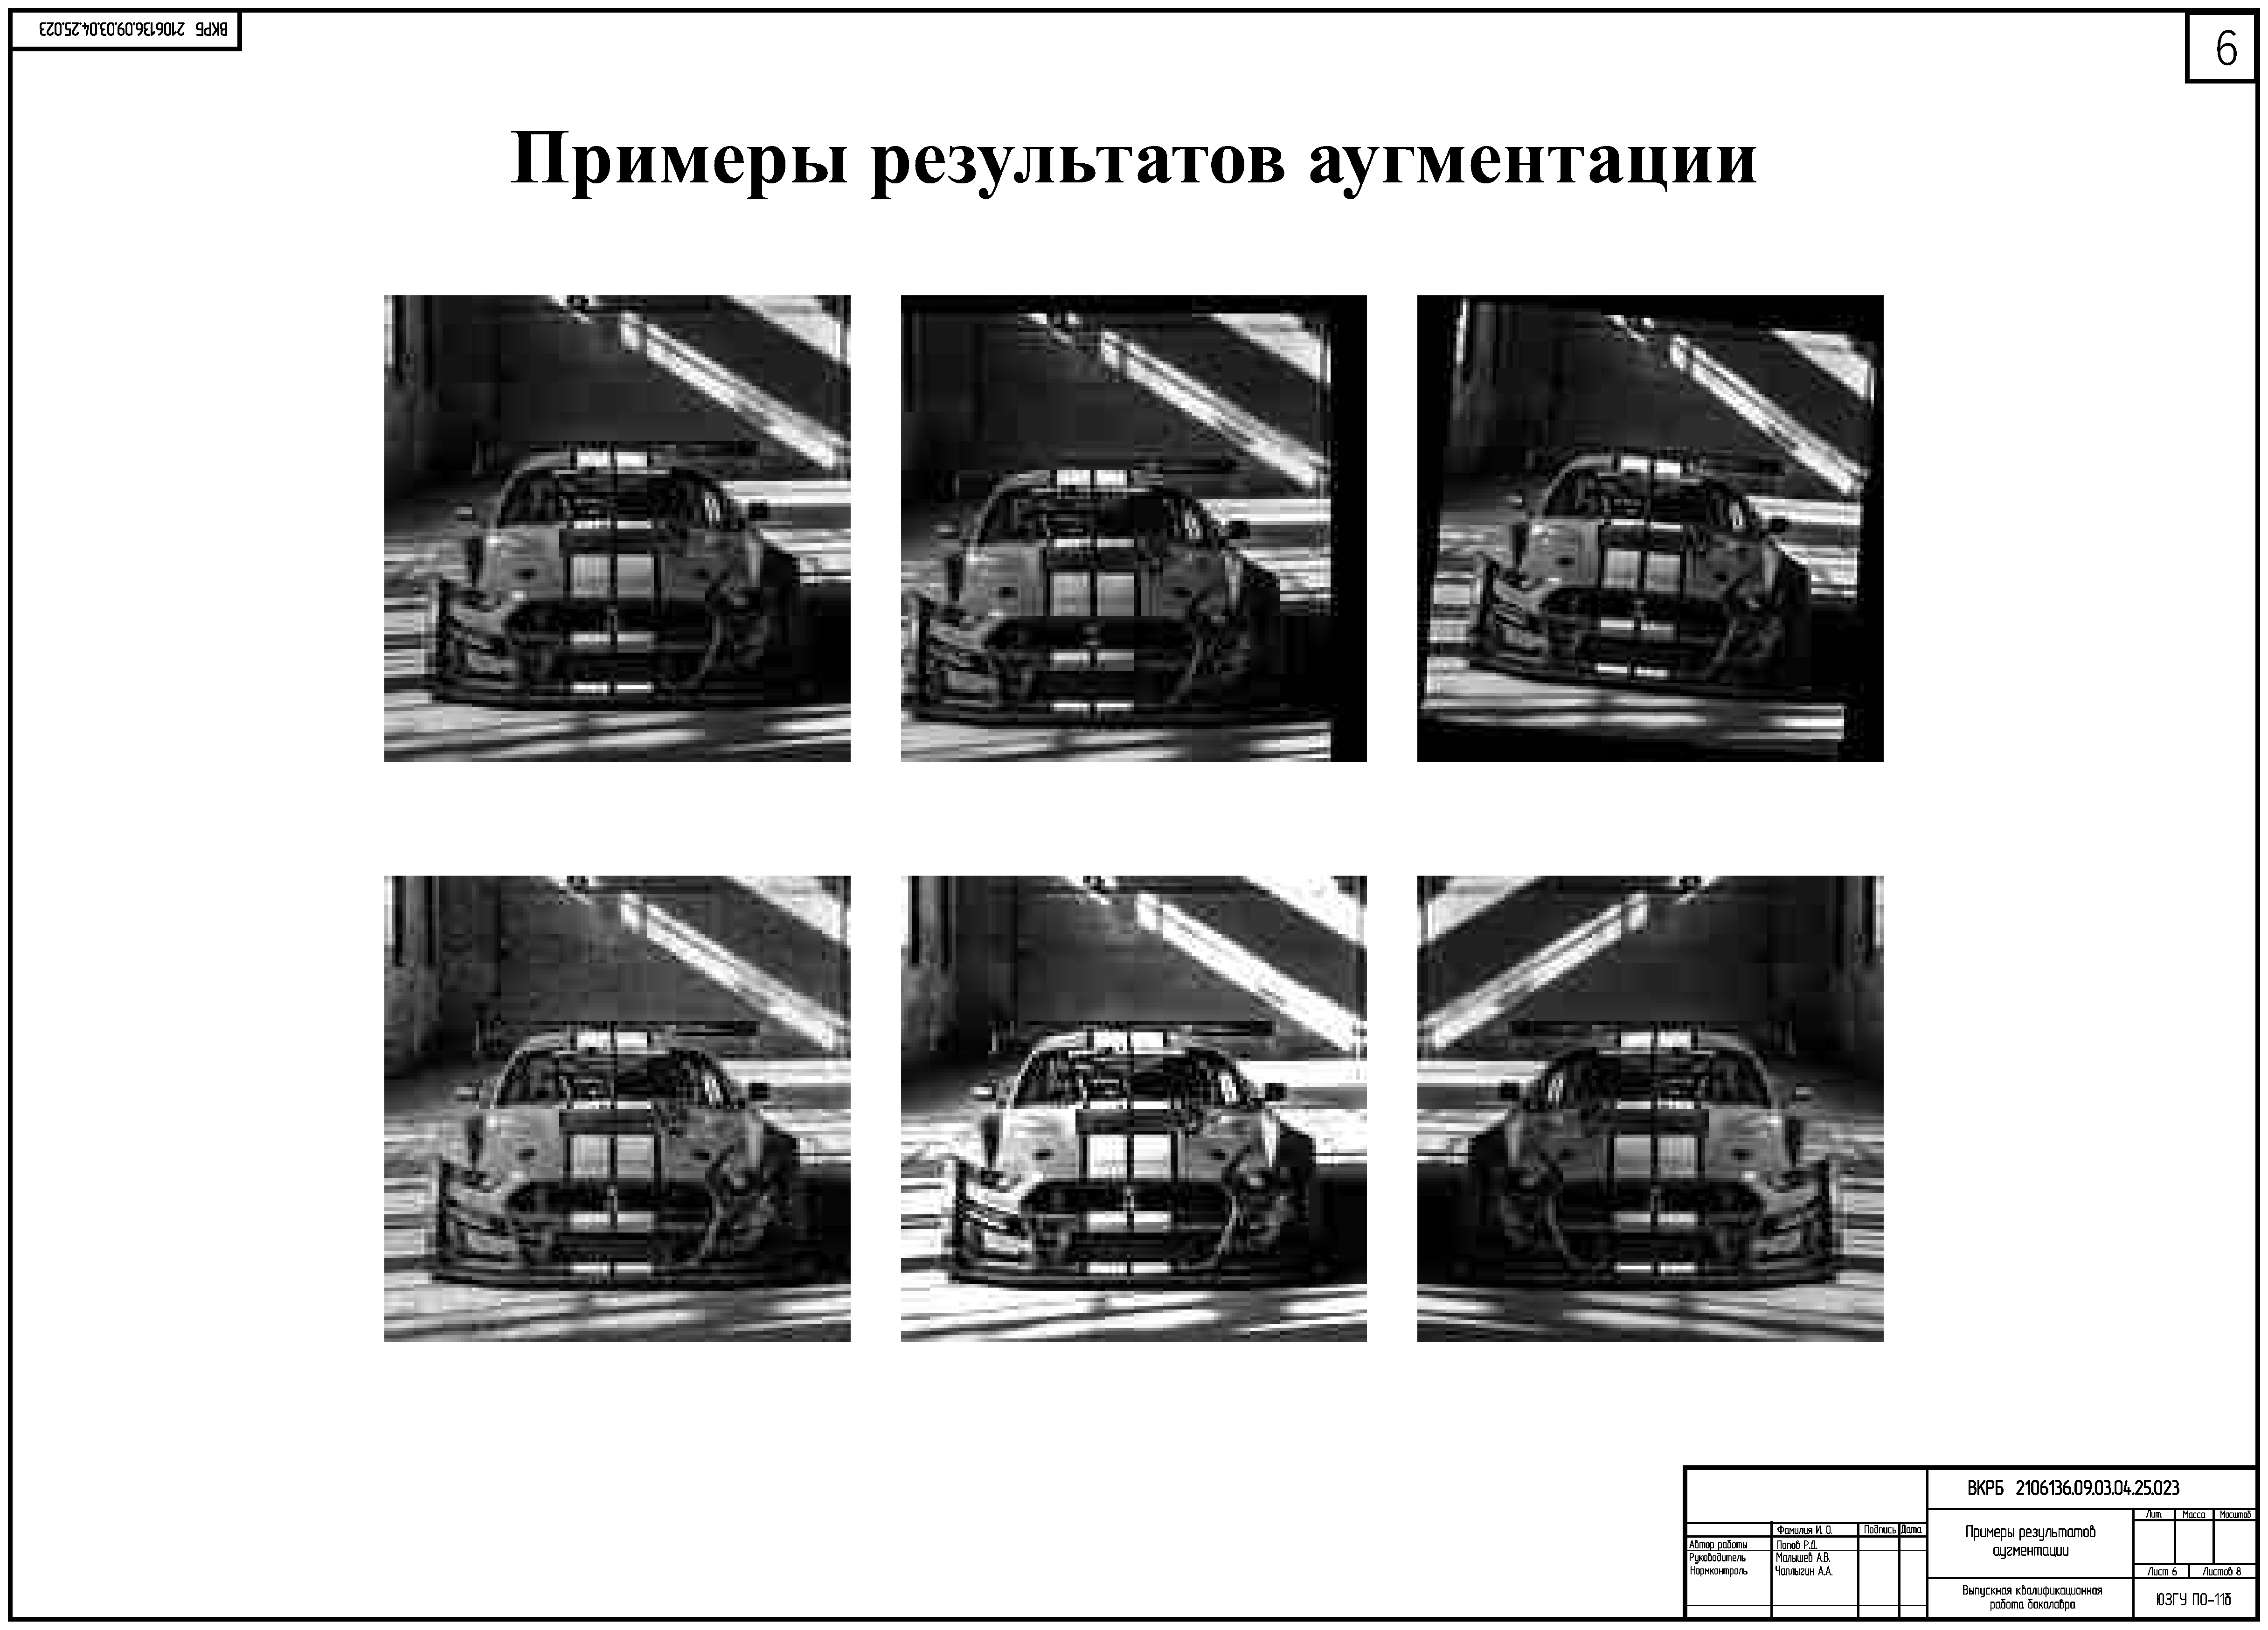
\includegraphics[width=0.82\linewidth]{list6.eps}
	\заголовок{Примеры результатов аугментации}
	\label{pl6:image}      
\end{плакат}

\begin{плакат}
	
\includegraphics[width=0.82\linewidth]{list7.eps}
	\заголовок{Интерфейс программы}
	\label{pl7:image}      
\end{плакат}

\begin{плакат}
	
\includegraphics[width=0.82\linewidth]{list8.eps}
	\заголовок{Заключение}
	\label{pl8:image}      
\end{плакат}


\end{landscape}
}\fi
\ifПрактика{}\else{\appendix{Фрагменты исходного кода программы}

main.tex
\lstinputlisting[language=Tex, frame=none]{main.tex}

ТехПроект.tex
\lstinputlisting[language=Tex, frame=none]{ТехПроект.tex}

\ifВКР{
\newpage
\addcontentsline{toc}{section}{На отдельных листах (CD-RW в прикрепленном конверте)}
\noindent
\begin{tabular}{p{5.8cm}C{4.8cm}C{4.8cm}}
   Автор ВКР & \lhrulefill{\fill} & \fillcenter\Автор \\
            \setarstrut{\footnotesize}
           & \footnotesize{(подпись, дата)} & \\
            \restorearstrut
   Руководитель ВКР & \lhrulefill{\fill} & \fillcenter\Руководитель \\
            \setarstrut{\footnotesize}
           & \footnotesize{(подпись, дата)} & \\
            \restorearstrut
   Нормоконтроль & \lhrulefill{\fill} & \fillcenter\Нормоконтроль \\
            \setarstrut{\footnotesize}
           & \footnotesize{(подпись, дата)} & \\
            \restorearstrut
\end{tabular}
\vskip 2cm
\begin{center}
\textbf{Место для диска}
\end{center}
}\fi
}\fi
\end{document}
